% !TeX program = xelatex
% !TeX TXS-program:compile = txs:///xelatex/[--shell-escape]
%%%%%%%%%%%%%%%%%%%%%%%%%%%%%%%%%%%%%%%%%%%%%%%%%%%%%%%%%%%%%%%%%%%%%%%%
% Plantilla TFG/TFM
% Escuela Politécnica Superior de la Universidad de Alicante
% Realizado por: Jose Manuel Requena Plens
% Contacto: info@jmrplens.com / Telegram:@jmrplens
%%%%%%%%%%%%%%%%%%%%%%%%%%%%%%%%%%%%%%%%%%%%%%%%%%%%%%%%%%%%%%%%%%%%%%%%

% Elige si deseas optimizar la ejecución del proyecto almacenando las figuras generadas con TikZ y PGF en una carpeta (archivos/figuras-procesadas).
% 1 - Si, 2 - No
\def\OptimizaTikZ{1}

% Archivo .TEX que incluye todas las configuraciones del documento y los paquetes. Añade todo aquello que necesites utilizar en el documento en este archivo.
% En él se encuentra la configuración de los márgenes, establecidos según las directrices de estilo de la EPS.
%%%%%%%%%%%%%%%%%%%%%%%%%%%%%%%%%%%%%%%%%%%%%%%%%%%%%%%%%%%%%%%%%%%%%%%%
% Plantilla TFG/TFM
% Escuela Politécnica Superior de la Universidad de Alicante
% Realizado por: Jose Manuel Requena Plens
% Contacto: info@jmrplens.com / Telegram:@jmrplens
%%%%%%%%%%%%%%%%%%%%%%%%%%%%%%%%%%%%%%%%%%%%%%%%%%%%%%%%%%%%%%%%%%%%%%%%

%%%%%%%%%%%%%%%%%%%%%%%%
% FORMATO DEL DOCUMENTO
%%%%%%%%%%%%%%%%%%%%%%%%
% scrbook es la clase de documento
% Si se desea que no haya página en blanco entre capítulos añadir "openany" en los parámetros de la clase. Sino siempre los capítulos empezarán en página impar.
\documentclass[a4paper,11pt,titlepage]{scrbook}
\KOMAoption{toc}{bib,chapterentryfill} % Opciones del índice
\usepackage{scrhack} % Previene algunos errores
% Paquete de formato para scrbook. Con marcas, linea-separador superior e inferior
\usepackage[automark,headsepline,footsepline]{scrlayer-scrpage}
\clearpairofpagestyles		% Borra los estilos por defecto
%%
% Formato y contenido de la información de cabecera y pie de página
%%
% Información de capítulo en cabecera e interno
\ihead{{\color{gray30}\scshape\small\headmark}}	
% Número de página en cabecera y externo
\ohead{\normalfont\pagemark} 
% Número de página en pie de página y externo. Sólo en páginas sin cabecera
\ofoot[\normalfont\pagemark]{}
%% 		
% Edición del contenido de las distintas partes de la cabecera
%%
\renewcommand{\chaptermark}[1]{\markboth{#1}{}} % Capítulo (Solo texto)
\renewcommand{\sectionmark}[1]{\markright{\thesection. #1}} % Sección (Número y texto)
\setkomafont{pagenumber}{} % Número de página (Sin nada añadido)

% Añade al índice y numera hasta la profundidad 4.
% 1:section,2:subsection,3:subsubsection,4:paragraph
\setcounter{tocdepth}{4}
\setcounter{secnumdepth}{4}
% Muestra una regla para comprobar el formato de las páginas
%\usepackage[type=upperleft,showframe,marklength=8mm]{fgruler}
% MÁRGENES DE LAS PÁGINAS
\usepackage[
  inner	=	3.0cm, % Margen interior
  outer	=	2.5cm, % Margen exterior
  top	=	2.5cm, % Margen superior
  bottom=	2.5cm, % Margen inferior
  includeheadfoot, % Incluye cabecera y pie de página en los márgenes
]{geometry}
% Valor de interlineado
\renewcommand{\baselinestretch}{1.0} % 1 línea de interlineado
% Para poder generar páginas horizontales
\usepackage{lscape}
% Ancho de la zona para comentarios en el margen. (modificado para todonotes)
\setlength{\marginparwidth}{1.9cm}

%%%%%%%%%%%%%%%%%%%%%%%%
% BIBLIOGRAFÍA
%%%%%%%%%%%%%%%%%%%%%%%%
\usepackage{apacite} % NORMA APA
\usepackage{natbib}
\usepackage{breakcites}

%%%%%%%%%%%%%%%%%%%%%%%%
% DOCUMENTO EN ESPAÑOL
%%%%%%%%%%%%%%%%%%%%%%%%
\usepackage[base]{babel}
\usepackage{polyglossia}
\setdefaultlanguage{spanish}

\addto\captionsspanish{%
	\renewcommand{\listtablename}{Índice de tablas} 
	\renewcommand{\tablename}{Tabla}
	\renewcommand{\lstlistingname}{Código}
	\renewcommand{\lstlistlistingname}{Índice de \lstlistingname s}
	\renewcommand{\glossaryname}{Glosario}
	\renewcommand{\acronymname}{Acrónimos}
	\renewcommand{\bibname}{Bibliografía}%
}

%%%%%%%%%%%%%%%%%%%%%%%% 
% COLORES
%%%%%%%%%%%%%%%%%%%%%%%% 
% Biblioteca de colores
\usepackage{color}
\usepackage[dvipsnames]{xcolor}
% Otros colores definidos por el usuario
\definecolor{gray97}{gray}{.97}
\definecolor{gray75}{gray}{.75}
\definecolor{gray45}{gray}{.45}
\definecolor{gray30}{gray}{.30}
\definecolor{negro}{RGB}{0,0,0}
\definecolor{blanco}{RGB}{255,255,255}
\definecolor{dkgreen}{rgb}{0,.6,0}
\definecolor{dkblue}{rgb}{0,0,.6}
\definecolor{dkyellow}{cmyk}{0,0,.8,.3}
\definecolor{gray}{rgb}{0.5,0.5,0.5}
\definecolor{mauve}{rgb}{0.58,0,0.82}
\definecolor{deepblue}{rgb}{0,0,0.5}
\definecolor{deepred}{rgb}{0.6,0,0}
\definecolor{deepgreen}{rgb}{0,0.5,0}
\definecolor{MyDarkGreen}{rgb}{0.0,0.4,0.0}
\definecolor{bluekeywords}{rgb}{0.13,0.13,1}
\definecolor{greencomments}{rgb}{0,0.5,0}
\definecolor{redstrings}{rgb}{0.9,0,0}

%%%%%%%%%%%%%%%%%%%%%%%%
% TABLAS
%%%%%%%%%%%%%%%%%%%%%%%%
% Paquetes para tablas
\usepackage{longtable,booktabs,array,multirow,multicol,tabularx,ragged2e,array}
% Nuevos tipos de columna para tabla, se pueden utilizar como por ejemplo C{3cm} en la definición de columnas de la función tabular
\newcolumntype{L}[1]{>{\raggedright\let\newline\\\arraybackslash\hspace{0pt}}m{#1}}
\newcolumntype{C}[1]{>{\centering\let\newline\\\arraybackslash\hspace{0pt}}m{#1}}
\newcolumntype{R}[1]{>{\raggedleft\let\newline\\\arraybackslash\hspace{0pt}}m{#1}}

%%%%%%%%%%%%%%%%%%%%%%%% 
% GRAFICAS y DIAGRAMAS 
%%%%%%%%%%%%%%%%%%%%%%%% 
% Paquete para todo tipo de gráficas, diagramas, modificación de imágenes, etc
\usepackage{tikz,tikzpagenodes}
\usetikzlibrary{tikzmark,calc,shapes.geometric,arrows,backgrounds,shadings,shapes.arrows,shapes.symbols,shadows,positioning,fit,automata,patterns,intersections}
\usepackage{pgfplots}
\pgfplotsset{colormap/jet}
\pgfplotsset{compat=newest} % Compatibilidad
\usepgfplotslibrary{patchplots,groupplots,fillbetween,polar}
\usepackage{pgfplotstable}
% Guardar las figuras realizadas con Tikz y Pgf en una carpeta externa
% para agilizar el procesado y tenerlas para utilizarlas en otros
% documentos
\if\OptimizaTikZ 1
\usepgfplotslibrary{external}
\tikzexternalize[prefix=archivos/figuras-procesadas/] % Ruta
\tikzset{%
    external/system call ={xelatex -enable-write18 -halt-on-error -interaction=batchmode -jobname "\image" "\texsource"},
}
\fi

% Estilos para elementos graficos
% Cajas y cajas de texto
\tikzstyle{Caja1} = [green,very thick,rounded corners,fill=white, fill opacity=0.5]
\tikzstyle{Texto1} = [fill=white,thick,shape=circle,draw=black,inner sep=2pt,font=\sffamily,text=black]
\tikzstyle{Texto2} = [fill=white,thick,shape=rectangle,draw=black,inner sep=2pt,font=\sffamily,text=black]
\tikzstyle{Texto3} = [fill=white,thick,shape=circle,draw=black,inner sep=2pt,font=\sffamily,text=black]
% Cuadros de diagrama
\tikzstyle{rectvioleta} = [rectangle, rounded corners, text centered, draw=black, fill=blue!10]
\tikzstyle{rectnaranja} = [rectangle, minimum width=2cm, minimum height=1cm, text centered, draw=black, fill=orange!10]
\tikzstyle{romborosa} = [diamond, aspect=3, minimum width=3cm, minimum height=1cm, text centered, draw=black, fill=red!10]
\tikzstyle{rectverde} = [rectangle, minimum width=2cm, minimum height=1cm, text centered, draw=black, fill=green!10]
\tikzstyle{rectamarillo} = [rectangle, rounded corners, minimum width=2cm, minimum height=1cm, text centered, draw=black, fill=yellow!10]
% Flechas
\tikzstyle{arrow} = [thick,->,>=stealth]

%%%%%%%%%%%%%%%%%%%%%%%% 
% FIGURAS, TABLAS, ETC 
%%%%%%%%%%%%%%%%%%%%%%%% 
\usepackage{subcaption} % Para poder realizar subfiguras
\usepackage{caption} % Para aumentar las opciones de diseño
% Nombres de figuras, tablas, etc, en negrita la numeración, todo con letra small
\captionsetup{labelfont={bf,small},textfont=small}
% Paquete para modificar los espacios arriba y abajo de una figura o tabla
\usepackage{setspace}
% Define el espacio tanto arriba como abajo de las figuras, tablas
\setlength{\intextsep}{5mm}
% Para ajustar tamaños de texto de toda una tabla o grafica
% Uso: {\scalefont{0.8} \begin{...} \end{...} }
\usepackage{scalefnt}
% Redefine las tablas y figuras para eliminar el '.' entre la numeración y el texto
\renewcommand*{\figureformat}{\figurename~\thefigure}
\renewcommand*{\tableformat}{\tablename~\thetable}

%%%%%%%%%%%%%%%%%%%%%%%% 
% TEXTO
%%%%%%%%%%%%%%%%%%%%%%%%
% Paquete para poder modificar las fuente de texto
\usepackage{xltxtra}
% Cualquier tamaño de texto. Uso: {\fontsize{100pt}{120pt}\selectfont tutexto}
\usepackage{anyfontsize}
% Para modificar parametros del texto.
\usepackage{setspace}
% Paquete para posicionar bloques de texto
\usepackage{textpos}
% Paquete para realizar cajas de texto. 
% Uso: \begin{mdframed}[linecolor=red!100!black] tutexto \end{mdframed}
\usepackage{framed,mdframed}
% Para subrayar. Uso: \hlc[tucolor]{tutexto}
\newcommand{\hlc}[2][yellow]{ {\sethlcolor{#1} \hl{#2}} }

%%%%%%%%%%%%%%%%%%%%%%%% 
% OTROS
%%%%%%%%%%%%%%%%%%%%%%%%
% Para hacer una pagina horizontal. Uso: \begin{landscape} xxxx \end{lanscape}
\usepackage{lscape} 
% Para incluir paginas PDF. Uso:
% \includepdf[pages={1}]{tuarchivo.pdf}
\usepackage{pdfpages}
% Para introducir url's con formato. Uso: \url{http://www.google.es}
\usepackage{url}
% Amplia muchas funciones graficas de latex
\usepackage{graphicx}
% Paquete que añade el hipervinculo en referencias dentro del documento, indice, etc
% Se define sin bordes alrededor. Uso: \ref{tulabel}
\usepackage[pdfborder={000}]{hyperref}
\usepackage{float}
\usepackage{placeins}
\usepackage{afterpage}
\usepackage{verbatim}
% Paquete para condicionales avanzados
\usepackage{xstring,xifthen}
% Paquete para realizar calculos en el código
\usepackage{calc}
% Para rotar tablas o figuras o su contenido
\usepackage{rotating} 
% Para incluir comentarios en el texto. El parámetro 'disable' oculta todas las notas.
% USO: \todo{tutexto}
\usepackage[textsize=tiny,spanish,shadow,textwidth=2cm]{todonotes}
%\reversemarginpar % Descomentar si se quiere todos los comentarios en el mismo lado
% Desactiva la exportación de los ToDo y Missingfigures como figuras
\if\OptimizaTikZ 1
\makeatletter
\renewcommand{\todo}[2][]{\tikzexternaldisable\@todo[#1]{#2}\tikzexternalenable}
\makeatother
\usepackage{letltxmacro}
\LetLtxMacro{\oldmissingfigure}{\missingfigure}
\makeatletter
\renewcommand{\missingfigure}[2][]{\tikzexternaldisable\oldmissingfigure[{#1}]{#2}\tikzexternalenable}
\makeatother
\fi

%%%%%%%%%%%%%%%%%%%%%%%% 
% GLOSARIOS
%%%%%%%%%%%%%%%%%%%%%%%%
\usepackage[acronym,nonumberlist,toc]{glossaries}
\usepackage{glossary-superragged}
\newglossarystyle{modsuper}{%
  \setglossarystyle{super}%
  \renewcommand{\glsgroupskip}{}
}
\renewcommand{\glsnamefont}[1]{\textbf{#1}}


%%%%%%%%%%%%%%%%%%%%%%%% 
% COMANDOS AÑADIDOS
%%%%%%%%%%%%%%%%%%%%%%%%
% Para mostrar la fecha actual (mes año) con \Hoy
\newcommand{\MES}{%
  \ifcase\month% 0
    \or Enero% 1
    \or Febrero% 2
    \or Marzo% 3
    \or Abril% 4
    \or Mayo% 5
    \or Junio% 6
    \or Julio% 7
    \or Agosto% 8
    \or Septiembre% 9
    \or Octubre% 10
    \or Noviembre% 11
    \or Diciembre% 12
  \fi}
\newcommand{\ANYO}{\number\year}
\newcommand{\Hoy}{\MES\ \ANYO}

%%%%%%%%%%%%%%%%%%%%%%%% 
% MATEMÁTICAS
%%%%%%%%%%%%%%%%%%%%%%%%
\usepackage{mathtools,amsthm,amsfonts,amssymb,bm,mathrsfs,nicefrac,upgreek,bigints} 
% Comando para añadir información de variables a las ecuaciones
% Uso: \begin{condiciones}[donde:] ....... \end{condiciones}
\newenvironment{condiciones}[1][2]
  {%
   #1\tabularx{\textwidth-\widthof{#1}}[t]{
     >{$}l<{$} @{}>{${}}c<{{}$}@{} >{\raggedright\arraybackslash}X
   }%
  }
  {\endtabularx\\[\belowdisplayskip]}

%%%%%
% PARÁMETROS DE FORMATO DE CODIGOS
%%%%%
% Puedes editar los formatos para ajustarlos a tu gusto
%%%%%%%%%%%%%%%%%%%%%%%%%%%%%%%%%%%%%%%%%%%%%%%%%%%%%%%%%%%%%%%%%%%%%%%%
% Plantilla TFG/TFM
% Escuela Politécnica Superior de la Universidad de Alicante
% Realizado por: Jose Manuel Requena Plens
% Contacto: info@jmrplens.com / Telegram:@jmrplens
%%%%%%%%%%%%%%%%%%%%%%%%%%%%%%%%%%%%%%%%%%%%%%%%%%%%%%%%%%%%%%%%%%%%%%%%


%%%%%%%%%%%%%%%%%%%%%%%% 
% CÓDIGO. CONFIGURACIÓN. En el siguiente bloque están los estilos.
%%%%%%%%%%%%%%%%%%%%%%%%
% Paquete para mostrar código de matlab. En caja y lineas numeradas
\usepackage[framed,numbered]{matlab-prettifier}
% Paquete mostrar código de programación de distintos lenguajes
\usepackage{listings}
\lstset{ inputencoding=utf8,
extendedchars=true,
frame=single, % Caja donde se ubica el código
backgroundcolor=\color{gray97}, % Color del fondo de la caja
rulesepcolor=\color{black},
boxpos=c,
abovecaptionskip=-4pt,
aboveskip=12pt,
belowskip=0pt,
lineskip=0pt,
framerule=0pt,
framextopmargin=4pt,
framexbottommargin=4pt,
framexleftmargin=11pt,
framexrightmargin=0pt,
linewidth=\linewidth,
xleftmargin=\parindent,
framesep=0pt,
rulesep=.4pt,
stringstyle=\ttfamily,
showstringspaces = false,
showspaces = false,
showtabs = false,
columns=fullflexible,
basicstyle=\small\ttfamily,
commentstyle=\color{gray45},
keywordstyle=\bfseries,
tabsize=4,
numbers=left,
numbersep=1pt,
numberstyle=\tiny\ttfamily\color{gray75},
numberfirstline = false,
breaklines=true,
postbreak=\mbox{\textcolor{red}{$\hookrightarrow$}\space}, % Flecha al saltar de linea
prebreak=\mbox{\textcolor{red}{$\hookleftarrow$}\space}, % Flecha al saltar de linea
literate=
  {á}{{\'a}}1 {é}{{\'e}}1 {í}{{\'i}}1 {ó}{{\'o}}1 {ú}{{\'u}}1
  {Á}{{\'A}}1 {É}{{\'E}}1 {Í}{{\'I}}1 {Ó}{{\'O}}1 {Ú}{{\'U}}1
  {à}{{\`a}}1 {è}{{\`e}}1 {ì}{{\`i}}1 {ò}{{\`o}}1 {ù}{{\`u}}1
  {À}{{\`A}}1 {È}{{\'E}}1 {Ì}{{\`I}}1 {Ò}{{\`O}}1 {Ù}{{\`U}}1
  {ä}{{\"a}}1 {ë}{{\"e}}1 {ï}{{\"i}}1 {ö}{{\"o}}1 {ü}{{\"u}}1
  {Ä}{{\"A}}1 {Ë}{{\"E}}1 {Ï}{{\"I}}1 {Ö}{{\"O}}1 {Ü}{{\"U}}1
  {â}{{\^a}}1 {ê}{{\^e}}1 {î}{{\^i}}1 {ô}{{\^o}}1 {û}{{\^u}}1
  {Â}{{\^A}}1 {Ê}{{\^E}}1 {Î}{{\^I}}1 {Ô}{{\^O}}1 {Û}{{\^U}}1
  {œ}{{\oe}}1 {Œ}{{\OE}}1 {æ}{{\ae}}1 {Æ}{{\AE}}1 {ß}{{\ss}}1
  {ű}{{\H{u}}}1 {Ű}{{\H{U}}}1 {ő}{{\H{o}}}1 {Ő}{{\H{O}}}1
  {ç}{{\c c}}1 {Ç}{{\c C}}1 {ø}{{\o}}1 {å}{{\r a}}1 {Å}{{\r A}}1
  {€}{{\euro}}1 {£}{{\pounds}}1 {«}{{\guillemotleft}}1
  {»}{{\guillemotright}}1 {ñ}{{\~n}}1 {Ñ}{{\~N}}1 {¿}{{?`}}1,
  }

% Intenta no dividir los códigos en diferentes paginas si es posible
\lstnewenvironment{listing}[1][]
   {\lstset{#1}\pagebreak[0]}{\pagebreak[0]}

% Formato de títulos de los códigos
\DeclareCaptionFont{white}{\color{white}}
\DeclareCaptionFormat{listing}{\colorbox{gray}{\parbox{\textwidth - 2\fboxsep}{#1#2#3}}}
\captionsetup[lstlisting]{format=listing,labelfont=white,textfont=white,font= scriptsize}


%%%%%%%%%%%%%%%%%%%%%%%% 
% CÓDIGO. ESTILOS. Ajústalos a tu gusto
%%%%%%%%%%%%%%%%%%%%%%%%
\lstdefinestyle{Consola}
	{
	basicstyle=\scriptsize\bf\ttfamily,
	}
   
\lstdefinestyle{C}
	{
	basicstyle=\scriptsize,
	language=C,
	}
\lstdefinestyle{C-color}
	{
  	breaklines=true,
  	language=C,
  	basicstyle=\scriptsize,
  	keywordstyle=\bfseries\color{green!40!black},
  	commentstyle=\itshape\color{purple!40!black},
  	identifierstyle=\color{blue},
  	stringstyle=\color{orange},
    }
\lstdefinestyle{CSharp}
	{
	basicstyle=\scriptsize
	language=[Sharp]C,
	escapeinside={(*@}{@*)},
	keywordstyle=\bfseries,
	}
\lstdefinestyle{CSharp-color}
	{
	basicstyle=\scriptsize
	language=[Sharp]C,
	escapeinside={(*@}{@*)},
	commentstyle=\color{greencomments},
	keywordstyle=\color{bluekeywords}\bfseries,
	stringstyle=\color{redstrings},
	}
\lstdefinestyle{C++}
	{
	basicstyle=\scriptsize,
	language=C++,
 	}
 	
\lstdefinestyle{C++-color}
	{
  	breaklines=true,
  	language=C++,
  	basicstyle=\scriptsize,
  	keywordstyle=\bfseries\color{green!40!black},
  	commentstyle=\itshape\color{purple!40!black},
  	identifierstyle=\color{blue},
  	stringstyle=\color{orange},
    }
    
\lstdefinestyle{PHP}
	{
	basicstyle=\scriptsize,
	language=PHP,
	}
	
\lstdefinestyle{PHP-color}
	{
	basicstyle=\scriptsize,
	language=PHP,
	keywordstyle    = \color{dkblue},
  	stringstyle     = \color{red},
  	identifierstyle = \color{dkgreen},
  	commentstyle    = \color{gray},
  	emph            =[1]{php},
  	emphstyle       =[1]\color{black},
  	emph            =[2]{if,and,or,else},
  	emphstyle       =[2]\color{dkyellow}
  }
  
\lstdefinestyle{Matlab}
	{
	basicstyle=\scriptsize,
	language=Matlab,
	numberstyle=\tiny\ttfamily\color{gray75},
	}
	
\lstdefinestyle{Matlab-color}
	{
	style = Matlab-editor,
	basicstyle=\scriptsize,
	numberstyle=\tiny\ttfamily\color{gray75},
	}
	
\lstdefinestyle{Latex}
	{
	language=[LaTeX]{Tex},
    basicstyle=\scriptsize,
    literate={\$}{{{\bfseries\$}}}1,
    alsoletter={\\,*,\&},
    emph =[1]{\\begin,\\end,\\caption,\\label,\\centering,\\FloatBarrier,
              \\lstinputlisting,\\scalefont,\\addplot,\\input,
              \\legend,\\item,\\subitem,\\includegraphics,\\textwidth,
              \\section,\\subsection,\\subsubsection,\\paragraph,
              \\cite,\\citet,\\citep,\\gls,\\bibliographystyle,\\url,
              \\citet*,\\citep*,\\todo,\\missingfigure,\\footnote},
  	emphstyle =[1]\bfseries,
  	emph = [2]{equation,subequations,eqnarray,figure,subfigure,
  			   condiciones,flalign,tikzpicture,axis,lstlisting,
  			   itemize,description
  			   },
  	emphstyle =[2]\bfseries,
    numbers=none,
	}
	
\lstdefinestyle{Latex-color}
	{
	language=[LaTeX]{Tex},
    basicstyle=\scriptsize,
    commentstyle=\color{dkgreen},
    identifierstyle=\color{black},
    literate={\$}{{{\bfseries\color{Dandelion}\$}}}1, % Colorea el simbolo dollar
    alsoletter={\\,*,\&},
    emph =[1]{\\begin,\\end,\\caption,\\label,\\centering,\\FloatBarrier,
              \\lstinputlisting,\\scalefont,\\addplot,\\input,
              \\legend,\\item,\\subitem,\\includegraphics,\\textwidth,
              \\section,\\subsection,\\subsubsection,\\paragraph,
              \\cite,\\citet,\\citep,\\gls,\\bibliographystyle,\\url,
              \\citet*,\\citep*,\\todo,\\missingfigure,\\footnote},
  	emphstyle =[1]\bfseries\color{RoyalBlue},
  	emph = [2]{equation,subequations,eqnarray,figure,subfigure,
  			   condiciones,flalign,tikzpicture,axis,lstlisting,
  			   itemize,description
  			   },
  	emphstyle =[2]\bfseries,
    numbers=none,
	}
\lstdefinestyle{Java}
{
	basicstyle=\scriptsize,
	language=Java,
}

\lstdefinestyle{Java-color}
{
	basicstyle=\scriptsize,
	language=Java,
  	keywordstyle=\color{blue},
  	commentstyle=\color{dkgreen},
  	stringstyle=\color{mauve},
}
\lstdefinestyle{Python}
{
	language=Python,
	basicstyle=\scriptsize,
	otherkeywords={self},  
	keywordstyle=\bfseries,     
	emphstyle=\bfseries,    
	emph={MyClass,__init__},         
}

\lstdefinestyle{Python-color}
{
	language=Python,
	basicstyle=\scriptsize,
	otherkeywords={self},          
	keywordstyle=\bfseries\color{deepblue},
	emph={MyClass,__init__},         
	emphstyle=\bfseries\color{deepred},    
	stringstyle=\color{deepgreen},
}
\lstdefinestyle{R}
{
	language=R,                     
  	basicstyle=\scriptsize,
  	keywordstyle=\bfseries, 
}
\lstdefinestyle{R-color}
{
	language=R,                     
  	basicstyle=\scriptsize,
  	keywordstyle=\bfseries\color{RoyalBlue}, 
  	commentstyle=\color{YellowGreen},
  	stringstyle=\color{ForestGreen}  
}


%%%%%
% DEFINICION DE CONCEPTOS
%%%%
% Uso ejemplo: \begin{ejemplo} tucontenido \end{ejemplo} 
\newtheorem{teorema}{Teorema}[chapter]
\newtheorem{ejemplo}{Ejemplo}[chapter]
\newtheorem{definicion}{Definición}[chapter]



%%%%%%%%%%%%%%%%%%%%%%%%%%%%%%%%%%%%%%%%%%%%%%%%%%%%%%%%%%%%%%%%%%%%%%
% INFORMACIÓN DEL TFG
% Comentar lo que NO se desee añadir y sustituir con la información correcta.
%%%%%%%%%%%%%%%%%%%%%%%%%%%%%%%%%%%%%%%%%%%%%%%%%%%%%%%%%%%%%%%%%%%%%%
% Título y subtítulo
\newcommand{\titulo}{Demo técnica para PC}
\newcommand{\subtitulo}{La demoscene}
% Datos del autor
\newcommand{\miNombre}{Luis González Aracil}
\newcommand{\miEmail}{lga42@alu.ua.es}
% Datos del tutor/es
\newcommand{\miTutor}{Francisco José Gallego Durán}
\newcommand{\departamentoTutor}{Ciencia de la Computación e Inteligencia Artificial}
% Datos de la facultada y universidad
\newcommand{\miFacultad}{Escuela Politécnica Superior}
\newcommand{\miFacultadCorto}{EPS UA}
\newcommand{\miUniversidad}{\protect{Universidad de Alicante}}
\newcommand{\miUbicacion}{Alicante}

%%%%%%%%%%%%%%%%%%%%%%%%%%%%%%%%%%%%%%%%%%%%%%%%%%%%%%%%%%%%%%%%%%%%%%
% INDICA TU TITULACIÓN
% ID	GRADO -------------------------------------------------
% 1		Ingeniería en Imagen y Sonido en Telecomunicación
% 2		Ingeniería Civil
% 3		Ingeniería Química
% 4		Ingeniería Informática
% 5		Ingeniería Multimedia
% 6		Arquitectura Técnica
% 7		Arquitectura
% 8		Robótica
% %		%%%%%%%%%%%%
% ID	MÁSTER ------------------------------------------------
% A		Telecomunicación
% B		Caminos, Canales y Puertos
% C		Gestión en la Edificación
% D		Desarrollo Web
% E		Materiales, Agua, Terreno
% F		Informática
% G 	Automática y Robótica
% H		Prevención de riesgos laborales
% I		Gestión Sostenible Agua
% J		Desarrollo Aplicaciones Móviles
% K		Ingeniería Química
%%%%%%%%%%%%%%%%%%%%%%%%%%%%%%%%%%%%%%%%%%%%%%%%%%%%%%%%%%%%%%%%%%%%%%%%%
%!!!!!!!!!!!!!!!!!!!!!!!!!!!!!!!!!!!!!!!!!!!!!!!!!!!!!!!!!!!!!!!!!!!!!%%%
																		%
\def\IDtitulo{5} % INTRODUCE LA ID DE TU TITULACIÓN						%
																		%
%!!!!!!!!!!!!!!!!!!!!!!!!!!!!!!!!!!!!!!!!!!!!!!!!!!!!!!!!!!!!!!!!!!!!!%%%
%%%%%%%%%%%%%%%%%%%%%%%%%%%%%%%%%%%%%%%%%%%%%%%%%%%%%%%%%%%%%%%%%%%%%%%%%

% Configuración automática según el identificador elegido
%%%%%%%%%%%%%%%%%%%%%%%%%%%%%%%%%%%%%%%%%%%%%%%%%%%%%%%%%%%%%%%%%%%%%%%%
% Plantilla TFG/TFM
% Escuela Politécnica Superior de la Universidad de Alicante
% Realizado por: Jose Manuel Requena Plens
% Contacto: info@jmrplens.com / Telegram:@jmrplens
%%%%%%%%%%%%%%%%%%%%%%%%%%%%%%%%%%%%%%%%%%%%%%%%%%%%%%%%%%%%%%%%%%%%%%%%

%%%%%%%%%%%%%%%%%%%%%%%% 
% COLORES DE GRADOS.
% Si el color de la titulación ha cambiado, modifícalo en las lineas siguientes.
%%%%%%%%%%%%%%%%%%%%%%%%
% Grados
\definecolor{teleco}{RGB}{32,2,116}			% Teleco
\definecolor{civil}{RGB}{201,56,140}			% Civil
\definecolor{quimica}{RGB}{41,199,255}		% Química
\definecolor{informatica}{RGB}{0,128,255}	% Informatica
\definecolor{multimedia}{RGB}{239,206,53}	% Multimedia
\definecolor{arquitecnica}{RGB}{0,179,148}	% Arquitectura técnica
\definecolor{arquitectura}{RGB}{181,0,0}		% Arquitectura
\definecolor{robotica}{RGB}{0,128,255}		% Robótica
% Másteres
\definecolor{masterteleco}{RGB}{32,2,116}	% Teleco
\definecolor{caminos}{RGB}{201,56,140}		% Caminos, Canales y Puertos
\definecolor{gestedif}{RGB}{50,120,50}		% Gestión Edificación
\definecolor{desweb}{RGB}{250,43,22}			% Desarrollo Web
\definecolor{mataguaterre}{RGB}{210,250,50}	% Materiales, Agua, Terreno
\definecolor{masterinfor}{RGB}{0,128,255}	% Informática
\definecolor{autorobo}{RGB}{83,145,201}		% Automática y Robótica
\definecolor{prevencion}{RGB}{0,100,0}		% Prevención Riesgos
\definecolor{gestionagua}{RGB}{7,138,197}	% Gestión Agua
\definecolor{moviles}{RGB}{121,11,21}		% Aplicaciones Móviles
\definecolor{masterquimica}{RGB}{41,199,255}	% Aplicaciones Móviles

% Logotipos comunes de todas las titulaciones
\newcommand{\logoFacultad}{include/logos-universidad/LogoEPSNegro}
\newcommand{\logoUniversidad}{include/logos-universidad/LogoUANegro}
\newcommand{\logoUniversidadPortada}{include/logos-universidad/LogoUABlanco}

% Colores generales
\definecolor{negro}{RGB}{0,0,0}
\definecolor{blanco}{RGB}{255,255,255}
%%%%%%%%%%%%%%%%%%%%%%%% 
% CONDICIONALES. SEGUN LA ID ELEGIDA EN EL .TEX PRINCIPAL
% Según el ID seleccionado en TFG_EPS_UA.tex se configurará el nombre de la titulación, logotipos y color.
% Si tu titulación no esta correctamente definida cambia las imágenes que se definen para tu titulación en las lineas de abajo
% Si deseas añadir mas titulaciones ve al final de este archivo
%%%%%%%%%%%%%%%%%%%%%%%%
% Grados
	\if\IDtitulo 1 % Teleco
		% Logos
		\newcommand{\logoFacultadPortada}{include/logos-universidad/LogoEPSBlanco}
		\newcommand{\logoGradoPortada}{include/logos-titulaciones/LogoTelecoBlanco}
		\newcommand{\logoGrado}{include/logos-titulaciones/LogoTelecoNegro}
		% Texto
		\newcommand{\miGrado}{Grado en Ingeniería en Sonido e Imagen en Telecomunicación}
		\newcommand{\tipotrabajo}{Trabajo Fin de Grado}
		% Color
		\newcommand{\colorgrado}{teleco}
		\newcommand{\colortexto}{blanco}
	\else \if\IDtitulo 2 % Civil
		\newcommand{\logoFacultadPortada}{include/logos-universidad/LogoEPSBlanco}
		\newcommand{\logoGradoPortada}{include/logos-titulaciones/LogoCivilBlanco}
		\newcommand{\logoGrado}{include/logos-titulaciones/LogoCivilNegro}
		% Texto
		\newcommand{\miGrado}{Grado en Ingeniería Civil}
		\newcommand{\tipotrabajo}{Trabajo Fin de Grado}
		% Color
		\newcommand{\colorgrado}{civil}
		\newcommand{\colortexto}{blanco}
	\else \if\IDtitulo 3 % Quimica
		% Logos
		\newcommand{\logoFacultadPortada}{include/logos-universidad/LogoEPSNegro}
		\newcommand{\logoGradoPortada}{include/logos-titulaciones/LogoQuimicaNegro}
		\newcommand{\logoGrado}{include/logos-titulaciones/LogoQuimicaNegro}
		% Texto
		\newcommand{\miGrado}{Grado en Ingeniería Química}
		\newcommand{\tipotrabajo}{Trabajo Fin de Grado}
		% Color
		\newcommand{\colorgrado}{quimica}
		\newcommand{\colortexto}{negro}
	\else \if\IDtitulo 4 % Informatica
		% Logos
		\newcommand{\logoFacultadPortada}{include/logos-universidad/LogoEPSBlanco}
		\newcommand{\logoGradoPortada}{include/logos-titulaciones/LogoInformaticaBlanco}
		\newcommand{\logoGrado}{include/logos-titulaciones/LogoInformaticaNegro}
		% Texto
		\newcommand{\miGrado}{Grado en Ingeniería Informática}
		\newcommand{\tipotrabajo}{Trabajo Fin de Grado}
		% Color
		\newcommand{\colorgrado}{informatica}
		\newcommand{\colortexto}{blanco}
	\else \if\IDtitulo 5 % Multimedia
		% Logos
		\newcommand{\logoFacultadPortada}{include/logos-universidad/LogoEPSNegro}
		\newcommand{\logoGradoPortada}{include/logos-titulaciones/LogoMultimediaNegro}
		\newcommand{\logoGrado}{include/logos-titulaciones/LogoMultimediaNegro}
		% Texto
		\newcommand{\miGrado}{Grado en Ingeniería Multimedia}
		\newcommand{\tipotrabajo}{Trabajo Fin de Grado}
		% Color
		\newcommand{\colorgrado}{multimedia}
		\newcommand{\colortexto}{negro}
	\else \if\IDtitulo 6 % Arquitectura Tecnica
		% Logos
		\newcommand{\logoFacultadPortada}{include/logos-universidad/LogoEPSBlanco}
		\newcommand{\logoGradoPortada}{include/logos-titulaciones/LogoArqTecnicaBlanco}
		\newcommand{\logoGrado}{include/logos-titulaciones/LogoArqTecnicaNegro}
		% Texto
		\newcommand{\miGrado}{Grado en Arquitectura Técnica}
		\newcommand{\tipotrabajo}{Trabajo Fin de Grado}
		% Color
		\newcommand{\colorgrado}{arquitecnica}
		\newcommand{\colortexto}{blanco}
	\else \if\IDtitulo 7 % Arquitectura
		% Logos
		\newcommand{\logoFacultadPortada}{include/logos-universidad/LogoEPSBlanco}
		\newcommand{\logoGradoPortada}{include/logos-titulaciones/LogoArquitecturaBlanco}
		\newcommand{\logoGrado}{include/logos-titulaciones/LogoArquitecturaNegro}
		% Texto
		\newcommand{\miGrado}{Grado en Arquitectura}
		\newcommand{\tipotrabajo}{Trabajo Fin de Grado}
		% Color
		\newcommand{\colorgrado}{arquitectura}
		\newcommand{\colortexto}{blanco}
	\else \if\IDtitulo 8 % Robotica
		% Logos
		\newcommand{\logoFacultadPortada}{include/logos-universidad/LogoEPSBlanco}
		\newcommand{\logoGradoPortada}{include/logos-titulaciones/LogoInformaticaBlanco}
		\newcommand{\logoGrado}{include/logos-titulaciones/LogoInformaticaNegro}
		% Texto
		\newcommand{\miGrado}{Grado en Ingeniería Robótica}
		\newcommand{\tipotrabajo}{Trabajo Fin de Grado}
		% Color
		\newcommand{\colorgrado}{robotica}
		\newcommand{\colortexto}{blanco}
% Másteres
	\else \if\IDtitulo A % Teleco
		% Logos
		\newcommand{\logoFacultadPortada}{include/logos-universidad/LogoEPSBlanco}
		\newcommand{\logoGradoPortada}{include/logos-titulaciones/LogoTelecoBlanco}
		\newcommand{\logoGrado}{include/logos-titulaciones/LogoTelecoNegro}
		% Texto
		\newcommand{\miGrado}{Máster Universitario en Ingeniería en Telecomunicación}
		\newcommand{\tipotrabajo}{Trabajo Fin de Máster}
		% Color
		\newcommand{\colorgrado}{masterteleco}
		\newcommand{\colortexto}{blanco}
	\else \if\IDtitulo B % Caminos, Canales y puertos
		% Logos
		\newcommand{\logoFacultadPortada}{include/logos-universidad/LogoEPSBlanco}
		\newcommand{\logoGradoPortada}{include/logos-titulaciones/LogoCivilBlanco}
		\newcommand{\logoGrado}{include/logos-titulaciones/LogoCivilNegro}
		% Texto
		\newcommand{\miGrado}{Máster Universitario en Ingeniería de Caminos, Canales y Puertos}
		\newcommand{\tipotrabajo}{Trabajo Fin de Máster}
		% Color
		\newcommand{\colorgrado}{caminos}
		\newcommand{\colortexto}{blanco}
	\else \if\IDtitulo C % Gestión Edificación
		% Logos
		\newcommand{\logoFacultadPortada}{include/logos-universidad/LogoEPSBlanco}
		\newcommand{\logoGradoPortada}{include/logos-titulaciones/LogoMasterEdificacionBlanco}
		\newcommand{\logoGrado}{include/logos-titulaciones/LogoMasterEdificacionNegro}
		\newcommand{\tipotrabajo}{Trabajo Fin de Máster}
		% Texto
		\newcommand{\miGrado}{Máster Universitario en Gestión de la Edificación}
		% Color
		\newcommand{\colorgrado}{gestedif}
		\newcommand{\colortexto}{blanco}
	\else \if\IDtitulo D % Desarrollo web
		% Logos
		\newcommand{\logoFacultadPortada}{include/logos-universidad/LogoEPSBlanco}
		\newcommand{\logoGradoPortada}{include/logos-titulaciones/LogoMasterDesarrolloBlanco}
		\newcommand{\logoGrado}{include/logos-titulaciones/LogoMasterDesarrolloNegro}
		% Texto
		\newcommand{\miGrado}{Máster Universitario en Desarrollo de Aplicaciones y Servicios Web}
		\newcommand{\tipotrabajo}{Trabajo Fin de Máster}
		% Color
		\newcommand{\colorgrado}{desweb}
		\newcommand{\colortexto}{blanco}
	\else \if\IDtitulo E % Materiales, Agua, Terreno
		% Logos
		\newcommand{\logoFacultadPortada}{include/logos-universidad/LogoEPSNegro}
		\newcommand{\logoGradoPortada}{include/logos-titulaciones/LogoMasterMaterialesNegro}
		\newcommand{\logoGrado}{include/logos-titulaciones/LogoMasterMaterialesNegro}
		% Texto
		\newcommand{\miGrado}{Máster Universitario en Ingeniería de los Materiales, del Agua y del Terreno}
		\newcommand{\tipotrabajo}{Trabajo Fin de Máster}
		% Color
		\newcommand{\colorgrado}{mataguaterre}
		\newcommand{\colortexto}{negro}
	\else \if\IDtitulo F % Informatica
		% Logos
		\newcommand{\logoFacultadPortada}{include/logos-universidad/LogoEPSBlanco}
		\newcommand{\logoGradoPortada}{include/logos-titulaciones/LogoInformaticaBlanco}
		\newcommand{\logoGrado}{include/logos-titulaciones/LogoInformaticaNegro}
		% Texto
		\newcommand{\miGrado}{Máster Universitario en Ingeniería Informática}
		\newcommand{\tipotrabajo}{Trabajo Fin de Máster}
		% Color
		\newcommand{\colorgrado}{masterinfor}
		\newcommand{\colortexto}{blanco}
	\else \if\IDtitulo G % Automática y Robótica
		% Logos
		\newcommand{\logoFacultadPortada}{include/logos-universidad/LogoEPSBlanco}
		\newcommand{\logoGradoPortada}{include/logos-titulaciones/LogoMasterRoboticaBlanco}
		\newcommand{\logoGrado}{include/logos-titulaciones/LogoMasterRoboticaNegro}
		% Texto
		\newcommand{\miGrado}{Máster Universitario en Automática y Robótica}
		\newcommand{\tipotrabajo}{Trabajo Fin de Máster}
		% Color
		\newcommand{\colorgrado}{autorobo}
		\newcommand{\colortexto}{blanco}
	\else \if\IDtitulo H % Prevención de riesgos laborales
		% Logos
		\newcommand{\logoFacultadPortada}{include/logos-universidad/LogoEPSBlanco}
		\newcommand{\logoGradoPortada}{include/logos-titulaciones/LogoMasterPrevencionBlanco}
		\newcommand{\logoGrado}{include/logos-titulaciones/LogoMasterPrevencionNegro}
		% Texto
		\newcommand{\miGrado}{Máster Universitario en Prevención de Riesgos Laborales}
		\newcommand{\tipotrabajo}{Trabajo Fin de Máster}
		% Color
		\newcommand{\colorgrado}{prevencion}
		\newcommand{\colortexto}{blanco}
	\else \if\IDtitulo I % Gestion Agua
		% Logos
		\newcommand{\logoFacultadPortada}{include/logos-universidad/LogoEPSNegro}
		\newcommand{\logoGradoPortada}{include/logos-titulaciones/LogoMasterAguaNegro}
		\newcommand{\logoGrado}{include/logos-titulaciones/LogoMasterAguaNegro}
		% Texto
		\newcommand{\miGrado}{Máster Universitario en Gestión Sostenible y Tecnologías del Agua}
		\newcommand{\tipotrabajo}{Trabajo Fin de Máster}
		% Color
		\newcommand{\colorgrado}{gestionagua}
		\newcommand{\colortexto}{negro}
	\else \if\IDtitulo J % Aplicaciones Móviles
		% Logos
		\newcommand{\logoFacultadPortada}{include/logos-universidad/LogoEPSBlanco}
		\newcommand{\logoGradoPortada}{include/logos-titulaciones/LogoMasterMovilesBlanco}
		\newcommand{\logoGrado}{include/logos-titulaciones/LogoMasterMovilesNegro}
		% Texto
		\newcommand{\miGrado}{Máster Universitario en Desarrollo de Software para Dispositivos Móviles}
		\newcommand{\tipotrabajo}{Trabajo Fin de Máster}
		% Color
		\newcommand{\colorgrado}{moviles}
		\newcommand{\colortexto}{blanco}
	\else \if\IDtitulo K % Quimica
		% Logos
		\newcommand{\logoFacultadPortada}{include/logos-universidad/LogoEPSNegro}
		\newcommand{\logoGradoPortada}{include/logos-titulaciones/LogoQuimicaNegro}
		\newcommand{\logoGrado}{include/logos-titulaciones/LogoQuimicaNegro}
		% Texto
		\newcommand{\miGrado}{Máster Universitario en Ingeniería Química}
		\newcommand{\tipotrabajo}{Trabajo Fin de Máster}
		% Color
		\newcommand{\colorgrado}{masterquimica}
		\newcommand{\colortexto}{negro}


	\fi \fi \fi \fi \fi \fi \fi \fi \fi \fi \fi \fi \fi \fi \fi \fi \fi \fi \fi
	
%%%%%%%%%%%%%%%%%%%%%%%%%%%%%%%%%%%%%%%%%%%%%%%%%%%%%%%%%%%%%%%%%%%%%%%%	
% ¿COMO AÑADIR MÁS TITULACIONES?
% Para añadir más titulaciones, se debe continuar el el formato de ID -> Titulacion.
% Justo encima de la linea donde hay muchos '\fi' se debe escribir el condicional y el contenido de este tal que:
%
%	\else \if\IDtitulo X % Titulacion con ID=X		
% 		% Logos
%		\newcommand{\logoFacultadPortada}{include/logos-universidad/LogoEPSBlanco}
%		\newcommand{\logoGradoPortada}{include/logos-titulaciones/logotitulacion}
%		\newcommand{\logoGrado}{include/logos-titulaciones/logotitulacion}
%		% Texto
%		\newcommand{\miGrado}{Grado en XXXXXXXX}
%		\newcommand{\tipotrabajo}{Trabajo Fin de XXXX}
%		% Color
%		\newcommand{\colorgrado}{XXXX}
%		\newcommand{\colortexto}{XXX}
%	
% Por último añadir a la linea que tiene muchos '\fi', otro '\fi'. Listo, ya podrás usar la nueva ID con la configuración añadida.
%%%%%%%%%%%%%%%%%%%%%%%%%%%%%%%%%%%%%%%%%%%%%%%%%%%%%%%%%%%%%%%%%%%%%%%%	




 

% Información añadida a las propiedades del archivo PDF.
\hypersetup{
pdfauthor = {\miNombre~(\miEmail)},
pdftitle = {\titulo},
}

%%
% Archivo de acrónimos
%%
\makeglossaries % Genera la base de datos de acrónimos
%%%%%%%%%%%%%%%%%%%%%%%%%%%%%%%%%%%%%%%%%%%%%%%%%%%%%%%%%%%%%%%%%%%%%%%%
% Plantilla TFG/TFM
% Escuela Politécnica Superior de la Universidad de Alicante
% Realizado por: Jose Manuel Requena Plens
% Contacto: info@jmrplens.com / Telegram:@jmrplens
%%%%%%%%%%%%%%%%%%%%%%%%%%%%%%%%%%%%%%%%%%%%%%%%%%%%%%%%%%%%%%%%%%%%%%%%

% Lista de acrónimos (se ordenan por orden alfabético automáticamente)

% La forma de definir un acrónimo es la siguiente:
% \newacronyn{id}{siglas}{descripción}
% Donde:
% 	'id' es como vas a llamarlo desde el documento.
%	'siglas' son las siglas del acrónimo.
%	'descripción' es el texto que representan las siglas.
%
% Para usarlo en el documento tienes 4 formas:
% \gls{id} - Añade el acrónimo en su forma larga y con las siglas si es la primera vez que se utiliza, el resto de veces solo añade las siglas. (No utilices este en títulos de capítulos o secciones).
% \glsentryshort{id} - Añade solo las siglas de la id
% \glsentrylong{id} - Añade solo la descripción de la id
% \glsentryfull{id} - Añade tanto  la descripción como las siglas

\newacronym{ieee}{IEEE}{Institute of Electrical and Electronics Engineers}
\newacronym{tfg}{TFG}{Trabajo Final de Grado}
\newacronym{tfm}{TFM}{Trabajo Final de Máster}
\newacronym{apa}{APA}{American Psychological Association}
\newacronym{asa}{ASA}{Acoustical Society of America}
\newacronym{adaa}{ADAA}{Asociación de Acústicos Argentinos}
\newacronym{aes}{AES}{Audio Engineering Society}
\newacronym{aas}{AAS}{Australian Acoustical Society}
\newacronym{csic}{CSIC}{Consejo Superior de Investigaciones Científicas}
\newacronym{eaa}{EAA}{European Acoustics Association}
\newacronym{ioa}{IOA}{Institute Of Acoustics}
\newacronym{ica}{ICA}{International Congress on Acoustics}
\newacronym{iiav}{IIAV}{International Institute of Acoustics and Vibration}
\newacronym{ince}{I-INCE}{International Institute of Noise Control Engineering}
\newacronym{isva}{ISVA}{International Seminar on Virtual Acoustics}
\newacronym{isra}{ISRA}{International Symposium on Room Acoustics}
\newacronym{sea}{SEA}{Sociedad Española de Acústica}
 % Archivo que contiene los acrónimos

%%%%%%%%%%%%%%%%%%%%%%%% 
% INICIO DEL DOCUMENTO
% A partir de aquí debes empezar a realizar tu TFG/TFM
%%%%%%%%%%%%%%%%%%%%%%%%
\begin{document}

% Números romanos hasta el mainmatter.
\frontmatter

% PORTADA
%%%%%%%%%%%%%%%%%%%%%%%%%%%%%%%%%%%%%%%%%%%%%%%%%%%%%%%%%%%%%%%%%%%%%%%%
% Plantilla TFG/TFM
% Escuela Politécnica Superior de la Universidad de Alicante
% Realizado por: Jose Manuel Requena Plens
% Contacto: info@jmrplens.com / Telegram:@jmrplens
%%%%%%%%%%%%%%%%%%%%%%%%%%%%%%%%%%%%%%%%%%%%%%%%%%%%%%%%%%%%%%%%%%%%%%%%

%%%%%%%%%%%%%%%%%%%%%%%%
% PORTADA - no modificar
%%%%%%%%%%%%%%%%%%%%%%%%
% Establece las fuentes de texto de la portada
% Helvetica LS Std Cond. Uso: {\FuenteTitulo tutexto}
\newfontfamily\FuenteTitulo{HelveticaLTStd-Cond}[Path=./include/fuentes/]  
% Helvetica. Uso: {\FuentePortada tutexto}
\newfontfamily\FuentePortada{Helvetica}[Path=./include/fuentes/]  

% Ignora los márgenes establecidos para el documento. Después de la portada en blanco y negro (portada_bn.tex) devuelve los márgenes establecidos en configuracioninicial.tex
\newgeometry{ignoreall,top=2cm,outer=2cm,inner=2cm}

% Tamaño por defecto de la fuente de texto para:
\def\FuenteTamano{55pt}	% Tamaño para el título del trabajo
\def\interlinportada{5.0} % Interlineado por defecto para el título
\def\TamTrabajo{20pt} 	% Tamaño para el tipo de trabajo (grado o máster)
\def\TamTrabajoIn{20pt} 	% Tamaño para el salto de línea después de tipo de trabajo
\def\TamOtros{12pt} 	% Tamaño para datos personales y fecha
\def\TamOtrosIn{1pt} 	% Tamaño para los saltos de línea en la info personal

% Según la longitud del título se determina un tamaño e interlineado para él
\StrLen{\titulo}[\longitudtitulo] % Cuenta los caracteres título
% Comprueba la longitud del título y según sea este determina unos valores nuevos
\ifthenelse{\longitudtitulo > 180}{
\def\FuenteTamano{35pt}		% Si es mayor a 180 caracteres tamaño de fuente 35pt
\def\interlinportada{3.5}} 	% Establece nuevo interlineado
{\ifthenelse{\longitudtitulo > 140}{
\def\FuenteTamano{40pt}		% Si es mayor a 140 caracteres tamaño de fuente 40pt
\def\interlinportada{4.0}} 	% Establece nuevo interlineado
{\ifthenelse{\longitudtitulo > 120}{
\def\FuenteTamano{50pt}		% Si es mayor a 120 caracteres tamaño de fuente 50pt
\def\interlinportada{4.5}} 	% Establece nuevo interlineado
{} % Si no, no modifica el tamaño
} }

\if\OptimizaTikZ 1
\tikzexternaldisable % Desactiva la exportación com figura
\fi 

% Inicio de portada
\begin{titlepage}
% Offset horizontal para toda la portada
\newlength{\centeroffset}
\setlength{\centeroffset}{-0.5\oddsidemargin}
\addtolength{\centeroffset}{0.5\evensidemargin}
\thispagestyle{empty}

% Fondo del color del grado
\pagecolor{\colorgrado}
% Logo de la facultad en la esquina superior derecha
\begin{tikzpicture}[remember picture,overlay]
   \node[anchor=north west,inner sep=0pt] at ($(current page.north west)+(13.65cm,-1.4cm)$)
              {\includegraphics[width=5.3cm]{\logoFacultadPortada}};
\end{tikzpicture}

% Titulo y subtitulo
\hspace{0pt}
\vfill
\hspace{-0.8cm}\begin{tabular}{L{18cm}}
\begin{spacing}{\interlinportada}
{\raggedleft{\FuenteTitulo\fontsize{\FuenteTamano}{110pt}\selectfont\color{\colortexto}\titulo}}
\vspace{-7em}
\end{spacing}
\end{tabular}
\hfill\linebreak\\
\begin{tabular}{lL{12cm}}
\raisebox{-.35\height}{\includegraphics[width=2cm]{\logoGradoPortada}} & \begin{spacing}{1.5}{\raggedleft{\FuentePortada\fontsize{20pt}{40pt}\selectfont\color{\colortexto}\miGrado}} \end{spacing}\\
\end{tabular}
\vspace{2cm}
\vfill
\hspace{0pt}
% Franja negra con logotipo 
\begin{tikzpicture}[overlay, remember picture, inner sep=0pt, outer sep=0pt]
  \fill [black] (current page.south west) rectangle (\paperwidth,\paperheight-26.4cm);
\node[anchor=south west,inner sep=0pt] at ($(current page.south west)+(13.2cm,1.6cm)$)
              {\includegraphics[width=6.2cm]{\logoUniversidadPortada}};
\end{tikzpicture}

% Información personal y fecha
\begin{textblock*}{\textwidth}(0.3cm,-2.35cm)% Ancho - Pos X,PosY
\noindent {\FuentePortada \fontsize{\TamTrabajo}{45pt}\selectfont\color{white}\tipotrabajo}
\\[\TamTrabajoIn] 
{\FuentePortada \fontsize{\TamOtros}{30pt}\selectfont\color{white} Autor:}
\\[\TamOtrosIn]
{\FuentePortada \fontsize{\TamOtros}{50pt}\selectfont\color{white}\miNombre}
\\[\TamOtrosIn]
{\FuentePortada \fontsize{\TamOtros}{30pt}\selectfont\color{white} Tutor/es:}
\\[\TamOtrosIn]
{\FuentePortada \fontsize{\TamOtros}{30pt}\selectfont\color{white}\miTutor}
\\[\TamOtrosIn]
\ifx\miTutorB\undefined \else {\FuentePortada \fontsize{\TamOtros}{30pt}\selectfont\color{white}\miTutorB} \fi
\\[\TamOtrosIn]\\[\TamOtrosIn]		
{\FuentePortada \fontsize{\TamOtros}{30pt}\selectfont\color{white}\Hoy}
\end{textblock*}


\end{titlepage}

\if\OptimizaTikZ 1
\tikzexternalenable % Reactiva la exportación como figura
\fi

\pagecolor{white}






 % Portada Color
%%%%%%%%%%%%%%%%%%%%%%%%%%%%%%%%%%%%%%%%%%%%%%%%%%%%%%%%%%%%%%%%%%%%%%%%
% Plantilla TFG/TFM
% Escuela Politécnica Superior de la Universidad de Alicante
% Realizado por: Jose Manuel Requena Plens
% Contacto: info@jmrplens.com / Telegram:@jmrplens
%%%%%%%%%%%%%%%%%%%%%%%%%%%%%%%%%%%%%%%%%%%%%%%%%%%%%%%%%%%%%%%%%%%%%%%%

\begin{titlepage}

% Márgenes de esta pagina modificados
\newgeometry{ignoreall,top=2cm,bottom=2cm}

% Offset horizontal para toda la portada
\setlength{\centeroffset}{-0.5\oddsidemargin}
\addtolength{\centeroffset}{0.5\evensidemargin}
\thispagestyle{empty}

% Titulo y subtitulo
\noindent\hspace*{\centeroffset}\begin{minipage}{\textwidth}
\centering
\begin{spacing}{1.5}{\huge\bfseries \titulo}\end{spacing}
\noindent\rule[-1ex]{\textwidth}{3pt}\\[3.5ex] % Linea
{\large\bfseries \subtitulo\\[4cm]}
\end{minipage}

% Relleno hasta la zona central
\vspace{2.5cm}

% Zona central. Autor y Tutores
\noindent\hspace*{\centeroffset}
\begin{minipage}{\textwidth}
\centering

\textbf{Autor}\\ {\miNombre}\\[2.5ex]
\textbf{Tutor/es}\\
{\normalsize \miTutor\\
\ifx\departamentoTutor\undefined \else \small\textit \departamentoTutor\\ \fi
\ifx\miTutorB\undefined \else \normalsize \miTutorB\\ \fi
\ifx\departamentoTutorB\undefined \else\small\textit \departamentoTutorB\\[2cm] \fi
}
\end{minipage}

% Relleno hasta la zona de abajo
\vspace*{\fill}

% Zona de abajo
\noindent\hspace*{\centeroffset}
\begin{minipage}{\textwidth}
\centering
\noindent\hspace*{\centeroffset}
\begin{center}
{\includegraphics[width=3cm]{\logoGrado}}\\
{\raggedleft\miGrado}
\end{center}
\vspace*{2em}
\centering
\noindent\hspace*{\centeroffset}
\begin{minipage}[l]{6cm}
\includegraphics[width=5cm]{\logoFacultad}
\end{minipage}
\begin{minipage}[r]{6cm}
\includegraphics[width=5cm]{\logoUniversidad}
\end{minipage}
\\[1cm]
ALICANTE, \Hoy
\end{minipage}


\end{titlepage}

% A partir de aquí aplica los márgenes establecidos en configuracioninicial.tex
\restoregeometry


 % Portada B/N

%%%%% PREAMBULO
% Incluye el .tex que contiene el preámbulo, agradecimientos y dedicatorias.
%%%%%%%%%%%%%%%%%%%%%%%%%%%%%%%%%%%%%%%%%%%%%%%%%%%%%%%%%%%%%%%%%%%%%%%%
% Plantilla TFG/TFM
% Escuela Politécnica Superior de la Universidad de Alicante
% Realizado por: Jose Manuel Requena Plens
% Contacto: info@jmrplens.com / Telegram:@jmrplens
%%%%%%%%%%%%%%%%%%%%%%%%%%%%%%%%%%%%%%%%%%%%%%%%%%%%%%%%%%%%%%%%%%%%%%%%

\chapter*{Resumen}

Para poder usar una herramienta en toda su capacidad y funcionalidad, es necesario conocerla a fondo. Con la complejidad creciente de los ordenadores, está apareciendo una tendencia por despreocuparse de los detalles del bajo nivel, considerando que los detalles de implementación no son o deberían ser parte del problema.\\

Este trabajo es, en primer lugar, una reivindicación de la importancia del bajo nivel. A lo largo del mismo, se tratará la subcultura informática de la \emph{demoscene}.\\

El \emph{demoscening} se originó a primeros de los años 80, con el auge de los primeros ordenadores personales, y su principal objetivo era el de crear demostraciones técnicas de gráficos y sonido por computador en tiempo real, buscando siempre resultados sorprendentes que consiguieran sobrepasar las limitaciones técnicas de las máquinas de la época. Eran por tanto demostraciones artísticas de ingenio y de conocimiento del bajo nivel.\\

A lo largo de este trabajo se explorarán algunas de las técnicas gráficas más comúnmente usadas en el mundo de la \emph{demoscene}, revisadas desde la actualidad. Se hará un análisis previo de cada una de estas técnicas, para a continuación proceder a su implementación y posterior optimización.
Además, para concluir, se hará una propuesta de una demo aplicando todos los conocimientos explorados previamente.

\chapter*{Abstract}
In order to be able to use a tool at its maximum capability and functionality, it's important to have an in-depth knowledge of it. Given the always increasing complexity of computers, there's a trend in software development to look away from low level implementation details, considering that these details should not be part of the problem's solution.\\

This essay pretends to emphasise the importance of the low level. Throughout this document, I will be writing about a computer's subculture called \emph{demoscene}.\\

The \emph{demoscene} originated back in the 80's, when personal computers' popularity was in a crest. \emph{Demosceners}' main goal was to create technical graphical demos in real time. These demos always tried to show off the abilities of the programmers, who tried to overcome the technical limitations of the machines at the time, with surprising results.\\

This document will explore and revise some of the graphical techniques that were commonly used by \emph{demosceners}. Before the implementation of every technique, an in-depth analysis will take place. After it, the result will be revised and optimized if possible. Furthermore, there will be a last proposal consisting on a final demo gathering all the knowledge previously exposed.

\chapter*{Motivación y objetivo general}

\thispagestyle{empty}
\vspace{1cm}

Hablando con un compañero del trabajo sobre el lenguaje ensamblador,
yo estaba intentando argumentarle su utilidad, a lo que él me contestó 
\emph{"Hoy en día, saber ensamblador es como saber latín"}.
Su afirmación zanjó el tema, pues a partir de ese momento no tuve ganas de
seguir discutiendo, pero me hizo reflexionar. ¿Es inútil el ensamblador?
¿Sirve para algo el bajo nivel?\\

Para mí, la pregunta \emph{"¿Para qué sirve saber ensamblador?"} es perfectamente equiparable a la pregunta "\emph{¿Para qué le sirve a un arquitecto conocer las herramientas y materiales con los que va a construir una casa?"}.\\

Si una edificación cayera por una mala elección del material de los cimientos por parte del arquitecto, no habría duda en a quién culpar. Nadie abogaría que la culpa no es del arquitecto porque no es su responsabilidad conocer las bases.
Sin embargo, hoy en día hay una enorme tendencia en el mundo del desarrollo software por menospreciar o infravalorar los cimientos de la programación, considerándolo algo arcaico y de carácter puramente didáctico, pero no
práctico.\\ 

Yo me opongo radicalmente a esta visión, no sólo porque estoy convencido de la importancia de conocer el bajo nivel, si no que también encuentro cierta belleza en él. Cómo instrucciones en apariencia tan simples pueden construir sistemas tan complejos. A ello, se suma una gran curiosidad por saber cómo las cosas están hechas, desde el principio.\\

Una de las cosas que encuentro más apasionantes de la computación es la capacidad de los ordenadores, máquinas inertes y carentes de inteligencia real -por el momento- para reproducir nuestra realidad a partir de modelos matemáticos.\\

Los gráficos por computador son, por lo general, complejos. Sin embargo, hoy en día es posible crear con un ordenador imágenes que parecen fotografías y son capaces de engañar al ojo humano.\\

El objetivo principal de este trabajo es ir a las raíces, y revisar algunas de las técnicas que se usaban en los orígenes de los gráficos por computador para, a partir de operaciones con bajo coste computacional, generar escenas complejas.

\cleardoublepage %salta a nueva página impar
%% Aquí va la dedicatoria si la hubiese. Si no, comentar la(s) linea(s) siguientes
%\chapter*{Agradecimientos\footnote{Por si alguien tiene curiosidad, este ``simpático'' agradecimiento está tomado de la ``Tesis de Lydia Chalmers'' basada en el universo del programa de televisión Buffy, la Cazadora de Vampiros.http://www.buffy-cazavampiros.com/Spiketesis/tesis.inicio.htm}
%}
%
%\thispagestyle{empty}
%\vspace{1cm}
%
%Este trabajo no habría sido posible sin el apoyo y el estímulo de mi colega y amigo, Doctor Rudolf Fliesning,  bajo cuya supervisión escogí este tema y comencé la tesis. Sr. Quentin Travers, mi consejero en las etapas finales del trabajo, también ha sido generosamente servicial, y me ha ayudado de numerosos modos, incluyendo el resumen del contenido de los documentos que no estaban disponibles para mi examen, y en particular por permitirme leer, en cuanto estuvieron  disponibles, las copias de los  recientes extractos de los diarios de campaña del Vigilante Rupert Giles y la actual Cazadora la señorita Buffy Summers, que se encontraron con William the Bloody en 1998, y por facilitarme el pleno acceso  a los diarios de anteriores Vigilantes relevantes a la carrera de William the Bloody.
%
%También me gustaría agradecerle al Consejo la concesión de Wyndham-Pryce como Compañero, el cual me ha apoyado durante mis dos años de investigación, y la concesión de dos subvenciones de viajes, una para estudiar documentos en los Archivos de Vigilantes sellados en Munich, y otra para la investigación en campaña en Praga. Me gustaría agradecer a Sr. Travers, otra vez, por facilitarme  la acreditación  de seguridad para el trabajo en los Archivos de Munich, y al Doctor Fliesning por su apoyo colegial y ayuda en ambos viajes de investigación.
%
%No puedo terminar sin agradecer a mi familia, en cuyo estímulo constante y amor he confiado a lo largo de mis años en la Academia. Estoy agradecida también a los ejemplos de mis  difuntos hermano, Desmond Chalmers, Vigilante en Entrenamiento, y padre, Albert Chalmers, Vigilante. Su coraje resuelto y convicción siempre me inspirarán, y espero seguir, a mi propio y pequeño modo, la noble misión por la que dieron sus vidas. 
%
%Es a ellos a quien dedico este trabajo.
%
%\cleardoublepage %salta a nueva página impar
%% Aquí va la dedicatoria si la hubiese. Si no, comentar la(s) linea(s) siguientes


\chapter*{}
\setlength{\leftmargin}{0.5\textwidth}
\setlength{\parsep}{0cm}
\addtolength{\topsep}{0.5cm}
\begin{flushright}
\small\em{
A mis padres, por estar ahí, siempre.\\
A mi hermana, por ser mi incordio y mi alegría.\\
A mi familia y amigos, por apoyarme y alegrarme los días.\\
\bigskip
A mi tutor,\\
por la visión que me ha dado sobre el mundo de la programación\\
y que tan valiosa es.\\
\bigskip
A Lola, por haber marcado la dirección cuando estábamos perdidos
}
\end{flushright}


\cleardoublepage %salta a nueva página impar
% Aquí va la cita célebre si la hubiese. Si no, comentar la(s) linea(s) siguientes
\chapter*{}
\setlength{\leftmargin}{0.5\textwidth}
\setlength{\parsep}{0cm}
\addtolength{\topsep}{0.5cm}
\begin{flushright}
\small\em{
If you give people\\
the choice of writing\\
good code or fast code,\\
there's something wrong.\\
Good code should be fast\\
}
\end{flushright}
\begin{flushright}
\small{
Bjarne Stroustrup
}
\end{flushright}
\setlength{\leftmargin}{0.5\textwidth}
\setlength{\parsep}{0cm}
\addtolength{\topsep}{0.5cm}
\begin{flushright}
\small\em{
When the whole world is silent,\\
even one voice becomes powerful.
}
\end{flushright}
\begin{flushright}
\small{
Malala Yousafzai
}
\end{flushright}
\cleardoublepage %salta a nueva página impar
 

% Incluye después del archivo anterior el indice y lista de figuras, tablas y códigos.
\tableofcontents	% Índice
\listoffigures		% Índice de figuras
\listoftables		% Índice de tablas
\lstlistoflistings	% Índice de códigos

% Inicia la numeración habitual.
\mainmatter

%%%%
% CONTENIDO. CAPÍTULOS DEL TRABAJO - Añade o elimina según tus necesidades
%%%%
%%%%%%%%%%%%%%%%%%%%%%%%%%%%%%%%%%%%%%%%%%%%%%%%%%%%%%%%%%%%%%%%%%%%%%%%
% Plantilla TFG/TFM
% Escuela Politécnica Superior de la Universidad de Alicante
% Realizado por: Jose Manuel Requena Plens
% Contacto: info@jmrplens.com / Telegram:@jmrplens
%%%%%%%%%%%%%%%%%%%%%%%%%%%%%%%%%%%%%%%%%%%%%%%%%%%%%%%%%%%%%%%%%%%%%%%%

\chapter{Introducción}

Sin saber muy bien cómo, hemos llegado a un punto en el que conocer las bases del funcionamiento de un computador nos parece algo obsoleto, e incluso arcaico. Tecnologías con 20 años de antigüedad se tachan de reliquias en un mundo que aún no cuenta un siglo de antigüedad.\\

El irrefrenable avance de la tecnología y se rapidez de evolución es innegable, pero a menudo, cuando se avanza muy rápido, también se pierde muy rápido.\\

La abstracción en el mundo de la computación ha sido un factor clave, de hecho es el factor que ha permitido que un set reducido de instrucciones como el que tienen los ordenadores sea capaz de realizar cálculos de los que un humano jamás podría. Abstraer el software y llevarlo hacia modelos más cercanos al ser humano ha permitido pensar más en términos de nuestra realidad y menos en términos de mover memoria y realizar sumas y restas. Y esto es bueno, si para realizar cualquier mínima tarea tuviéramos que preocuparnos de hasta el más mínimo detalle de implementación, la curva de aprendizaje sería demasiado inclinada, y la eficiencia de la producción del software caería en picado.\\

Sin embargo, a más nos alejamos del hardware y más capas de abstracción añadimos, las instrucciones que escribimos se alejan más y más del reducido set de instrucciones que nuestro ordenador puede ejecutar. Como dijo una vez David J. Wheeler, \emph{"Todo problema en computación puede resolverse con otra capa de indirección, excepto el problema de tener demasiada indirección"}\footnote{\url{http://www.stroustrup.com/bs_faq.html}}. 

\section{La demoscene}

Void


\chapter{Introducción (Con ejemplos de contenido)}

Antes de comenzar la lectura de este documento debo agradecer el trabajo realizado por Pedro Pernías Peco en su plantilla de ``tfg'' que se puede ver en \url{https://github.com/lcg51/tfg}. Gracias a esa plantilla me he lanzado a crear mi versión. Algunos contenidos aquí mostrados han sido extraídos de la plantilla de Pedro. 
\\
\par Esta plantilla se ha diseñado de 0 y por ello no utiliza la misma estructura que la plantilla de Pedro. Pero la estructura de contenido para un TFG/TFM es la misma y a continuación se muestran las diferentes partes que debe tener un TFG/TFM redactado por Pedro.
\section{¡Importante!, leer primero}

Este texto está escrito pensando en orientar a los alumnos que usarán \LaTeX~para escribir su \gls{tfg} y \gls{tfm}. 
\\
\par Contiene información útil para aquellos que no tengan experiencia previa en \LaTeX~así como algunos datos acerca de cómo escribir mejor su \gls{tfg}.
A continuación, se ofrece una copia de la información que hay en el libro de estilo para la realización de los \gls{tfg} de la EPS de la Universidad de Alicante.

En los capítulos siguientes encontrarás ejemplos de muchas de las cosas que se pueden realizar con \LaTeX. Con un poco de paciencia, estudia cómo se hacen estas cosas y luego aplícalas en tus documentos.


\section{Estructura de un \glsentryshort{tfg}}

En caso de que el \gls{tfg}/\gls{tfm} tenga como finalidad la elaboración de un proyecto o un 
informe científico o técnico, deberá ajustarse a lo dispuesto en las normas UNE 
157001:2002 y UNE 50135:1996 respectivamente.

Si el \gls{tfg}/\gls{tfm} tiene por finalidad la elaboración de un trabajo monográfico, el 
documento presentado deberá constar de las siguientes partes, teniendo como base la 
norma UNE 50136:1997.

\begin{description}
\item[Preámbulo:] se describirán brevemente la motivación que ha originado la realización del \gls{tfg}/\gls{tfm}, así como una breve descripción de los objetivos generales que se quieren alcanzar con el trabajo presentado.
\item[Agradecimientos:] se podrán añadir las hojas necesarias para realizar los agradecimientos, a veces obligatorios, a las entidades y organismos colaboradores.
\item[Dedicatoria:] se podrá añadir una única hoja con dedicatorias, su alineación será derecha.
\item[Citas:] (frases célebres) se podrá añadir una única hoja con citas, su alineación será derecha.
\item[Índices:] cada índice debe comenzar en una nueva página, se incluirán los índices que se estimen necesarios (conforme UNE 50111:1989), en este orden:
\begin{description}
\item[Índice de contenidos:] (obligatorio siempre) se incluirá un índice de las secciones de las que se componga el documento, la numeración de las 
divisiones y subdivisiones utilizarán cifras arábigas (según UNE 50132:1994) y harán mención a la página del documento donde se ubiquen.
\item[Índice de figuras:] si el documento incluye figuras se podrá incluir también un índice con su relación, indicando la página donde se ubiquen.
\item[Índice de tablas:] en caso de existir en el texto, ídem que el anterior.
\item[Índice de abreviaturas, siglas, símbolos, etc.:] en caso de ser necesarios se podrán incluir cada uno de ellos.
\end{description}
\item[Cuerpo del documento:] en el contenido del documento se da flexibilidad para su organización y se puede estructurar en las secciones que se considere. En todo caso obligatoriamente se deberá, al menos, incluir los siguientes contenidos:
\begin{description}
\item[Introducción:] donde se hará énfasis a la importancia de la temática, su vigencia y actualidad; se planteará el problema a investigar, así como el propósito o finalidad de la investigación.
\item[Marco teórico o Estado del arte:] se hará mención a los elementos conceptuales que sirven de base para la investigación, estudios previos relacionados con el problema planteado, etc.
\item[Objetivos:] se establecerán el objetivo general y los específicos.
\item[Metodología:] se indicarán el tipo o tipos de investigación, las técnicas y los procedimientos que serán utilizados para llevarla a cabo; se identificarán la población y el tamaño de la muestra así como las técnicas e instrumentos de recolección de datos.
\item[Resultados:] incluirá los resultados de la investigación o trabajo, así como el análisis y la discusión de los mismos.
\end{description}
\item[Conclusiones:] obligatoriamente se incluirá una sección de conclusiones donde se realizará un resumen de los objetivos conseguidos así como de los resultados obtenidos si proceden.
\item[Bibliografía y referencias:] se incluirá también la relación de obras y materiales consultados y empleados en la elaboración de la memoria del \gls{tfg}/\gls{tfm}. La bibliografía y las referencias serán indexadas en orden alfabético (sistema nombre y fecha) o se numerará correlativamente según aparezca (sistema numérico). Se empleará la familia 1 como tipo de letra. Podrá utilizarse cualquier sistema bibliográfico normalizado predominante en la rama de conocimiento, estableciéndose como prioritarios el sistema ISO 690, sistema \gls{apa}  o Harvard (no necesariamente en ese orden de preferencia). En esta plantilla Latex se propone usar el estilo \gls{apa} indicándolo en la línea correspondiente como 
\begin{verbatim}
\bibliographystyle{apacite}
\end{verbatim}


\item[Anexos:] se podrán incluir los anexos que se consideren oportunos.

\end{description}

\section{Apartados dentro de los capítulos}
En \LaTeX~existen diferentes niveles de títulos para realizar secciones, subsecciones, etc. En esta web puedes ver más información al respecto \url{https://en.wikibooks.org/wiki/LaTeX/Document_Structure}

Para ello se utilizan los siguientes comandos;

\begin{lstlisting}[style=Latex-color]
	\section{Esto es una sección}
	Y este el contenido de la sección.
	\subsection{Esto es una subsección}
	Y este el contenido de la subsección.
	\subsubsection{Esto es una subsubsección}
	Y este el contenido de la subsubsección.
	\paragraph{Esto es un paragraph}
 	Y este el contenido del paragraph. Que siempre se inicia en la misma línea que el título del mismo.
\end{lstlisting}
 Y se genera lo siguiente:
 \section{Esto es una sección}
	Y este el contenido de la sección.
	\subsection{Esto es una subsección}
	Y este el contenido de la subsección.
	\subsubsection{Esto es una subsubsección}
	Y este el contenido de la subsubsección.
	\paragraph{Esto es un paragraph}
 	Y este el contenido del paragraph. Que siempre se inicia en la misma línea que el título del mismo.

\section{Citar bibliografía}
Para citar la bibliografía tal como se define en el sistema APA (en esta web se indica como debe aparecer en el texto la cita: \url{http://guides.libraries.psu.edu/apaquickguide/intext}) se debe realizar con alguno de los comandos mostrados a continuación:

\begin{lstlisting}[style=Latex-color]
Esto es una cita estándar: \citet{Shaw1996}, que también puedes mostrar con paréntesis así: \citep{Shaw1996}. También se puede realizar una cita indicando a qué parte te refieres \citep[ver][Cap. 2]{Shaw1996} o \citep[Cap. 2]{Shaw1996} o \citep[ver][]{Shaw1996}. 

También puedes mostrar todos los autores cuando hay más de 2 autores añadiendo un asterisco después del comando como: \citet*{Akyildiz2005}, sin el asterisco quedaría así: \citet{Akyildiz2005}.

O puedes citar dos o más fuentes al mismo tiempo: \citep{Barkan1995,Leighton2012}

\end{lstlisting}
Y \LaTeX~genera lo siguiente:
\\
\par Esto es una cita estándar: \citet{Shaw1996}, que también puedes mostrar con paréntesis así: \citep{Shaw1996}. También se puede realizar una cita indicando a qué parte te refieres \citep[ver][Cap. 2]{Shaw1996} o \citep[Cap. 2]{Shaw1996} o \citep[ver][]{Shaw1996}. 
\\
\par También puedes mostrar todos los autores cuando hay más de 2 autores añadiendo un asterisco después del comando como: \citet*{Akyildiz2005}, sin el asterisco quedaría así: \citet{Akyildiz2005}.
\\
\par O puedes citar dos o más fuentes al mismo tiempo: \citep{Barkan1995,Leighton2012}


\section{Notas a pie de página}

Para introducir notas a pie de página se debe escribir lo siguiente:

\begin{lstlisting}[style=Latex-color]
	La plantilla necesita el motor XeLaTeX \footnote{Para más información sobre XeLaTeX visita \url{https://es.sharelatex.com/learn/XeLaTeX}} (el más recomendable actualmente), por lo que si el programa que utilizas compila la plantilla con el motor pdfLaTeX \footnote{También puedes buscar más información en internet} (el más habitual pero menos potente) debes cambiarlo por XeLaTeX en las opciones del programa. Si no sabes como hacerlo busca en el manual del programa o en google.
\end{lstlisting}

\LaTeX~genera lo siguiente (observa las notas a pie de página):
\\
\par La plantilla necesita el motor XeLaTeX\footnote{Para más información sobre XeLaTeX visita \url{https://es.sharelatex.com/learn/XeLaTeX}} (el más recomendable actualmente), por lo que si el programa que utilizas compila la plantilla con el motor pdfLaTeX\footnote{También puedes buscar más información en internet} (el más habitual pero menos potente) debes cambiarlo por XeLaTeX en las opciones del programa. Si no sabes como hacerlo busca en el manual del programa o en google.
\section{Estilos de texto}

A continuación se muestran ejemplos de distintos estilos de texto:

\begin{itemize}
	\item \textbackslash textit\{Cursiva\} $\rightarrow$ \textit{Cursiva}
	\item \textbackslash emph\{Cursiva 2\} $\rightarrow$ \emph{Cursiva 2}
	\item \textbackslash textbf\{Negrita\} $\rightarrow$ \textbf{Negrita}
	\item \textbackslash texttt\{Monoespacio\} $\rightarrow$ \texttt{Monoespacio}
	\item \textbackslash textsc\{Mayúsculas capitales\} $\rightarrow$ \textsc{Mayúsculas capitales}
	\item \textbackslash uppercase\{Todo mayúsculas\} $\rightarrow$ \uppercase{Todo mayúsculas} 
\end{itemize}

 \section{Acrónimos}
 Ahora vamos a ver cómo se ponen los acrónimos.
 
 La norma dice que la primera vez que aparece un acrónimo debe ponerse su fórmula completa, es decir lo que significa, al lado del acrónimo. Después de ello, podemos usar sólo el acrónimo salvo cuando consideremos que debemos volver a usar la fórmula completa por alguna razón de legibilidad.
 
 ¿Cómo llevar la cuenta de cuándo es la primera vez que ponemos el acrónimo? si hacemos cambios en el doc es fácil que perdamos esa información así que lo mejor es que sea el propio \LaTeX~el que lleve esa cuenta. Para ello tenemos que hacer dos cosas:
 \begin{description}
 \item[Primero:] creamos la entrada del acrónimo en el fichero acronimos.tex. Revisa los comentarios de su cabecera para saber cómo crear esa entrada. Básicamente lo que hacemos allí es poner la ``fórmula corta'' y la ``fórmula larga'' del acrónimo es decir, el propio acrónimo y su significado
 \item[Segundo:] escribimos en el texto el acrónimo SIEMPRE diciendo que es un acrónimo y el tipo de fórmula que queremos usar. Por ejemplo, si siempre que queremos hacer referencia al IEEE escribimos \begin{lstlisting}[style=Latex-color]
 \gls{ieee}
 \end{lstlisting}  se consigue que la primera vez que aparezca el acrónimo ponga las fórmulas larga y corta y en las siguientes ocasiones sólo aparecerá la corta.
 \end{description}
 
 Aquí va un ejemplo:
 
 Si escribimos:
 
\begin{lstlisting}[style=Latex-color]
 El \gls{ieee} es una institución muy importante en el mundo de la
 ingeniería.  El \gls{ieee} lleva marcando normas y protocolos desde
 hace mucho tiempo.  Pero el \gls{ieee} no está solo en esta tarea. 
 Además del \gls{ieee} hay muchas otras instituciones para ello.  \end{lstlisting}
 
 Obtendremos: 
 
El \gls{ieee} es una institución muy importante en el mundo de la
 ingeniería.  El \gls{ieee} lleva marcando normas y protocolos desde
 hace mucho tiempo.  Pero el \gls{ieee} no está solo en esta tarea. 
 Además del \gls{ieee} hay muchas otras instituciones para ello.
 
 \section{Tareas por hacer}
 
 En esta plantilla se ha incluido un paquete para incluir notas/comentarios en el texto para recordar partes que hay que revisar o terminar de desarrollar. El uso es sencillo, el manual para conocer todos los comandos se encuentra en \url{http://osl.ugr.es/CTAN/macros/latex/contrib/todonotes/todonotes.pdf}, a continuación se muestran algunos ejemplos:
 \\
\par Para incluir un comentario sobre el texto:

\begin{lstlisting}[style=Latex-color]
	Recomiendo utilizar programas LaTeX que permitan trabajar con sistema de archivos para poder editar el conjunto de capítulos en la misma ventana. Este tipo de función lo tienen programas como TexStudio, es multiplataforma. \todo{Incluir más ejemplos de programas}
\end{lstlisting}

\LaTeX~genera lo siguiente:
\\
\par Recomiendo utilizar programas LaTeX que permitan trabajar con sistema de archivos para poder editar el conjunto de capítulos en la misma ventana. Este tipo de función lo tienen programas como TexStudio, es multiplataforma. \todo{Incluir más ejemplos de programas}
\vspace{1em}
\noindent\hrule
\vspace{1em}
\par Para incluir un comentario sobre el texto pero dentro del texto:

\begin{lstlisting}[style=Latex-color]
	Recomiendo utilizar programas LaTeX que permitan trabajar con sistema de archivos para poder editar el conjunto de capítulos en la misma ventana. Este tipo de función lo tienen programas como TexStudio, es multiplataforma. \todo[inline]{Incluir más ejemplos de programas}
\end{lstlisting}

\LaTeX~genera lo siguiente:
\\
\par Recomiendo utilizar programas LaTeX que permitan trabajar con sistema de archivos para poder editar el conjunto de capítulos en la misma ventana. Este tipo de función lo tienen programas como TexStudio, es multiplataforma. \todo[inline]{Incluir más ejemplos de programas}
\vspace{1em}
\noindent\hrule
\vspace{1em}
\par También se puede dejar indicado donde falta una imagen o figura, para incluirla más adelante del siguiente modo:

\begin{lstlisting}[style=Latex-color]
\missingfigure{Añadir gráfica de rendimiento}	
\end{lstlisting}

\LaTeX~genera lo siguiente:
\\
\missingfigure{Añadir gráfica de rendimiento}	



	% Plantilla: Se muestran contenidos
%%%%%%%%%%%%%%%%%%%%%%%%%%%%%%%%%%%%%%%%%%%%%%%%%%%%%%%%%%%%%%%%%%%%%%%%
% Plantilla TFG/TFM
% Escuela Politécnica Superior de la Universidad de Alicante
% Realizado por: Jose Manuel Requena Plens
% Contacto: info@jmrplens.com / Telegram:@jmrplens
%%%%%%%%%%%%%%%%%%%%%%%%%%%%%%%%%%%%%%%%%%%%%%%%%%%%%%%%%%%%%%%%%%%%%%%%

\chapter{Estado del arte}

\section{La demoscene}

\subsection{Qué es la demoscene}

La \emph{demoscene} es una subcultura informática cuyo principal objetivo es la creación de demostraciones técnicas llamadas \emph{demoscenes}. Una \emph{demoscene} es un programa autocontenido y por norma general de peso ligero que intenta explotar al máximo el \emph{software} y el \emph{hardware} de la máquina que la ejecuta, con el fin de generar efectos visuales y sonoros. El objetivo de una \emph{demoscene} suele consistir en mostrar el ingenio y las habilidades del programador, así como tratar de impresionar al público.\\

Además, aunque el \emph{demoscening} en sí mismo no se puede considerar una forma de arte, sí que es cierto que muchas demos poseen un cierto componente artístico.\\ 

Se distinguen principalmente dos tipos de demo\footnote{\url{http://www.oldskool.org/demos/explained/demo_reference.html}}:

\begin{itemize}
  \item \textbf{Demo}: programa que genera gráficos y sonido en tiempo real. Suele tener una extensión superior a 5 minutos y normalmente no tienen límite de tamaño. Una demo suele ser creada por un grupo de personas que incluye al menos un programador, un diseñador gráfico y un músico. Las demos actuales suelen estar realizadas en 3D y cuentan con aceleración gráfica por hardware. Las demos más antiguas o realizadas para plataformas más antiguas (conocidas como "demos \emph{oldskool}") son procesadas de forma íntegra por la CPU (pues las plataformas para las que se desarrollan no poseen GPU) y suelen combinar ilusiones 3D con efectos gráficos en 2D.
  \item \textbf{Intro}: una demo de corta duración. Una intro suele ser temática (mientras que una demo suele compilar distintas escenas/temáticas). Además, las intros no suelen superar los 5 minutos de duración y su tamaño tiende a estar restringido. Las principales categorías de intros son 64K (65536 bytes), 4K (4096 bytes) y 1K (1024 bytes).
\end{itemize}

Existen otras categorías de demo, aunque son mucho menos comunes, como las \textbf{mega demos} (demos de gran duración/extensión, compuestas por múltiples partes) o las \textbf{dentros} (intros cuyo propósito es ofrecer un avance de una demo por llegar, todavía en desarrollo).\\

Además, existen muchas otras categorías derivadas o relacionadas con la \emph{demoscene}, como la creación de gráficos procedimentales. Una de las subcategorías más populares dentro de esta son las \textbf{4K images}, imágenes complejas y de alta resolución generadas procedimentalmente por programas de 4096 bytes. También es posible encontrar categorías similares relacionadas con la generación procedimental de archivos de música o vídeo. Las mayores diferencias entre estas producciones y las demos son su tiempo de ejecución (no se ejecutan en tiempo real) y las técnicas que usan (al no ser el tiempo una limitación, pueden usar algoritmos computacionalmente más costosos, pero que generan resultados más complejos).

\subsection{Orígenes de la demoscene}

A principios de los años 80, con la popularización de los primeros ordenadores personales, la computación dejó de ser algo que sucedía en universidades para pasar a abrirse al gran mercado. Con ello, llegó también la distribución del software, aunque en aquella época no se producía por internet, si no tan sólo por medios físicos, como los disquetes. Estos programas venían con protecciones de copia por parte de los desarrolladores para evitar su distribución ilegal. Poco tardaron, no obstante, en aparecer los primeros \emph{crackers}, personas que se dedicaban a eliminar las protecciones de copia del software para su distribución gratuita. Esto llevó a la creación de una subcultura informática basada en el \emph{cracking} de videojuegos y otros tipos de software, al margen de la legalidad. Esto se hacía no solo con la intención de poder ditribuir el software de forma gratuita, si no que también suponía una fuente de diversión y competición para los \emph{crackers}\footnote{\url{https://web.archive.org/web/20170726063815/http://tomaes.32x.de/text/faq.php\#2.3}}.\\

Es por ello que los denominados \emph{crackers} empezaron a "firmar" el software que \emph{crackeaban} con seudónimos que aparecían en los menús o en las intros de los juegos. Con el tiempo, la competición y la ambición de los \emph{crackers} fue aumentando, y llegó un punto en el que no solo se limitaban a quitar las protecciones de copia del software, si no que también creaban sus propias intros para los programas.\\

Es en este punto cuando la \emph{demoscene} empieza a tomar forma, cuando una parte de los \emph{crackers} deciden retornar a la legalidad pero sin dejar atrás la competición y la diversión. De este modo, este nuevo sector se empieza a dedicar a la creación de intros y demos cuyo objetivo es mostrar sus habilidades al resto de \emph{demosceners}\footnote{\url{http://widerscreen.fi/assets/reunanen-wider-1-2-2014.pdf}}.

\subsection{Composición y cultura de la demoscene}

La \emph{demoscene} es una subcultura informática muy centrada en el trabajo en equipo y en compartir. Con el desarrollo y popularización de la \emph{demoscene}, a partir de principios de los 90 se popularizó y se estandarizó, con la creación de eventos y competiciones.\\

Heredado de las \emph{copyparties}, eventos en los que \emph{crackers} y \emph{demosceners} se juntaban para conocerse y compartir software, al margen de la legalidad, nuevos eventos empezaron a crearse a principios de los noventa. Estos eventos sí eran legales y se centraban únicamente en el aspecto de las demos. Pasan a ser eventos sociales en los que los \emph{demosceners} se conocen, comparten y compiten.\\

Estos eventos, conocidos como \emph{demoparties}, pasan entonces a ser concursos y tener distintas categorías y premios. Para concursar, normalmente los competidores se juntaban en grupos, usualmente compuestos por al menos un programador, un diseñador gráfico y un músico. Estos grupos tenían su propio nombre e identidad. A su vez, cada uno de los componentes del grupo también solía usar un seudónimo. El uso de un seudónimo es una herencia de los orígenes de la \emph{demoscene} en el \emph{cracking}, aunque el propósito de usar un alias cambia. Mientras que los \emph{crackers} usaban un nombre falso para ocultar su identidad, pues realizaban actividades ilegales, los \emph{demosceners} usan este alias como una forma de expresión.

\subsection{La demoscene en la actualidad}

Si bien la \emph{demoscene} siempre se ha mantenido como una subcultura y nunca ha llegado a tener una popularidad masiva, su auge se dio en los años noventa.  En la actualidad, muchos de los eventos de \emph{demoscening} que se crearon en los 90 han desaparecido, y otros tantos han derivado en eventos dedicados a los ordenadores de forma mucho más genérica, derivando en eventos de software o en \emph{LAN-parties}.\\

Del mismo modo que muchas ferias y eventos han desaparecido, muchos otros también se han ido creando. No obstante, parece que hay una tendencia general hacia el olvido.\\

Las \emph{demoparties} en la actualidad suelen ser eventos locales, normalmente humildes, donde participan apasionados y nostálgicos.\\

Es difícil atribuir las causas de la lenta caída en popularidad de la \emph{demoscene}, aunque hay varios factores que pueden contribuir a ello, del mismo modo que hay una serie de factores que evitan que se pierda.\\

Por un lado, la \emph{demoscene} es cada vez más pequeña debido a:

\begin{itemize}
  \item Siempre ha sido una subcultura, y nunca ha destacado especialmente por encima de otras subculturas informáticas.
  \item Para poder participar en la \emph{demoscene} hace falta una gran cantidad de conocimiento matemático y de programación de bajo nivel, cualidades que no abundan.
  \item Con el auge de los ordenadores, otro tipo de espacios más accesibles al público como las ferias tecnológicas, las ferias de videojuegos o las ferias de programación han eclipsado parcialmente a la \emph{demoscene}.
  \item Una parte de los \emph{demosceners} eran reacios a la incorporación de gente nueva e inexperta a la \emph{demoscene}, pues si bien aportaban sangre nueva, sus metas y conocimiento se alejaban de los originales de la escena.
\end{itemize}

Todos estos factores han contribuido a colocar la \emph{demoscene} como una práctica de nicho. Quizá una crítica válida sería que no ha sabido adaptarse de forma conveniente a los nuevos tiempos. El mundo de la \emph{demoscene} no ha sabido publicitarse o venderse suficientemente bien como para llegar a ser conocido por un público mayor. Sin embargo, la \emph{demoscene} sigue viva, y estos son algunos de los factores que contribuyen a ello:

\begin{itemize}
	\item El auge de lo \emph{retro}. En esta última década ha empezado a masivizarse un cierto reconocimiento y nostalgia hacia los orígenes de la computación y del videojuego. La popularización de los juegos \emph{indie}, técnicas como el \emph{pixel art} y tributos a videojuegos antiguos han llevado a destapar obras olvidadas y a suscitar un nuevo interés por todo lo \emph{retro}.
	\item La pasión y dedicación de los \emph{demosceners}, que siguen produciendo y compartiendo su obra, extendiendo así su pasión y abriéndola al público general.
	\item La masivización de la informática. Hoy en día hay muchísimos más informáticos que en los años 80 y 90. Si bien es cierto que hay una tendencia de abandono hacia el bajo nivel, también hay mucha más gente que se hace preguntas, investiga y se interesa por el mismo.
\end{itemize}

Como reflexión final me gustaría añadir que creo que es posible mantener el panorama de la \emph{demoscene} vivo, pero pienso que esto va a ser muy complicado si no se intenta abrir al público, cosa que algunas \emph{demoparties} ya están haciendo. Está claro que al abrir la \emph{demoscene} al público general se pierden cosas por el camino, y se gana gente que tiene un interés mucho más casual y mucho menos pasional. Creo que en el panorama actual esa gente es necesaria. No todo el mundo tiene el tiempo o la capacidad como para meterse de lleno en la \emph{demoscene}, pero hay muchas personas que sí pueden tener curiosidad por ella de una forma mucho más básica, y esta gente también cuenta. Cada vez es más común encontrar en ferias de videojuegos puestos \emph{retro}, y hay incluso museos del videojuego. La nostalgia y la veneración por los orígenes se abre paso, y pienso que es en este lugar donde la \emph{demoscene} puede buscar su camino.

\section{Eventos de demoscening}

A continuación se listan y describen brevemente algunas \emph{demosparties} que aún se celebran en la actualidad, en el año 2019.

\begin{itemize}
	\item \textbf{Revision}: tiene lugar en durante Pascua, en Alemania. Es la sucesora de la \emph{demoparty} Breakpoint\footnote{\url{http://breakpoint.untergrund.net}}. El evento se estableció en 2011, tras el fin de Breakpoint, y mantiene a muchos de los organizadores. El evento congrega a más de 800 personas de todo el mundo cada año, y es el mayor evento dedicado exclusivamente a la \emph{demoscene} en el mundo \footnote{\url{https://2019.revision-party.net}}.
	\item \textbf{Assembly} [\ref{fig:assembly}]: tiene lugar en verano en Finlandia, y es el mayor evento de \emph{demoscening} en el país. Además, es uno de las \emph{demoparties} más antiguas que siguen en activo, cumpliendo 25 años el pasado 2017. Sin embargo, el evento no está dedicado exclusivamente a la \emph{demoscene}, si no que es también un evento de videojuegos y \emph{esports}. No obstante, la \emph{demoscene} sigue siendo importante en él, y se celebran anualmente concursos en 5 categorías distintas (Demo, Oldskool demo, 64K intro, 4K intro y 1K intro)\footnote{\url{https://www.assembly.org/summer19/demoscene}}.
	\item \textbf{VIP (Very Important Party)}: es la \emph{demoparty} más longeva de Francia, cumpliendo este año su 20 aniversario. Congrega a personas de todas partes de Europa, aunque es una \emph{demoparty} principlamente francesa\footnote{\url{https://en.wikipedia.org/wiki/Very_Important_Party}}. Fue fundada por el grupo de \emph{demosceners} \emph{PoPsY TeAm}\footnote{\url{http://www.popsyteam.org}}.
	\item \textbf{Nova}: esta \emph{demoparty} fue creada en 2017, por lo que este año se celebra su tercera edición. Es la mayor \emph{demoparty} en Reino Unido, con una salón principial con capacidad para hasta cien \emph{demosceners}\footnote{\url{http://www.novaparty.org}}.
	\item  \textbf{Alternative Party}: es uno de los eventos de \emph{demoscening} más grandes de Finlandia. Es un festival bastante peculiar, (o alternativo, como su nombre indica) y su objetivo es motivar a los programadores y artistas a explorar su creatividad y nuevos puntos de vista. Suele mezclar ordenadores de distintas épocas y capacidades. Aunque mantiene una categoría constante a la mejor demo, el resto de categorías y premios cambian cada año, suponiendo así un reto aún mayor para los programadores. Ha tenido distintos invitados célebres dentro del mundo de la informática, como Al Lowe, creador del juego \emph{Leisure Suit Larry}. Además, la primera noche del evento incluye un concierto de música en el que participan artistas del mundo de la \emph{demoscene}. Este año se celebra su 20 aniversario\footnote{\url{http://www.altparty.org}}. 
	\item \textbf{Chaos Constructions}: es el festival de \emph{demoscenes} más longevo y popular que se celebra en Rusia. Tiene lugar en verano y se creó en 1995, aunque en aquel momento se llamada \emph{Enlight}. La celebración de esta \emph{demoparty} en el año 1997 congregó a más de 1200 personas. En la actualidad, su temática se ha ampliado, incluyendo nuevas areas como exposiciones y charlas empresariales. En 2018, el festival tuvo lugar durante dos días sin interrupción, contó con participantes internacionales y se emitió de forma íntegra por \emph{Twicht}\footnote{\url{https://chaosconstructions.ru/en/}}
\end{itemize}

\begin{figure}[h]
	\centering
	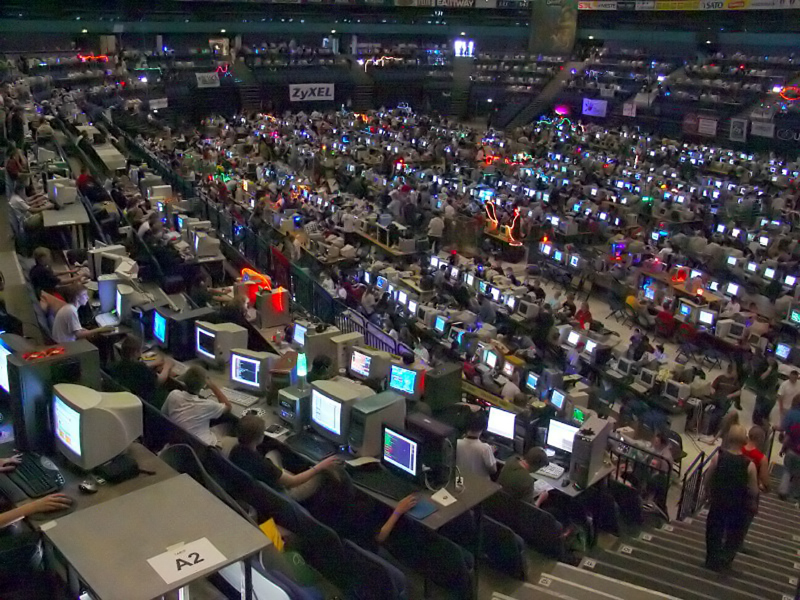
\includegraphics[width=10cm]{archivos/Assembly2004}
	\caption{Assembly 2004 - Fuente: \href{https://en.wikipedia.org/wiki/Demoscene\#/media/File:Assembly2004-areena01.jpg}{Wikipedia}}
	\label{fig:assembly}
\end{figure}

\section{Grupos de demoscening}

A continuación se listan y describen brevemente algunos de los grupos de \emph{demosceners} más populares.

\subsection{Farbrausch}

Farbraush es un grupo de \emph{demosceners} de origen alemán que empezó a ser notado a partir de diciembre del 2000, con su octava producción, llamada \emph{fr-08: .the .product}\footnote{\url{http://www.farbrausch.de/prod&which=17.py}}.\\

El nombre del grupo se puede traducir como "éxtasis de color". Todos sus proyectos empiezan por "fr-número\_del\_proyecto", donde el número del proyecto se decide en el momento de empezar a trabajar en el mismo, independientemente de cuándo se produzca su lanzamiento.\\

Farbraush tiene un gran cantidad de demos notorias, como Debris [\ref{fig:debris}], que está considerada en el popular portal \emph{demoscener} \url{http://www.pouet.net} como la mejor demo de todos los tiempos.

\begin{figure}[h]
	\centering
	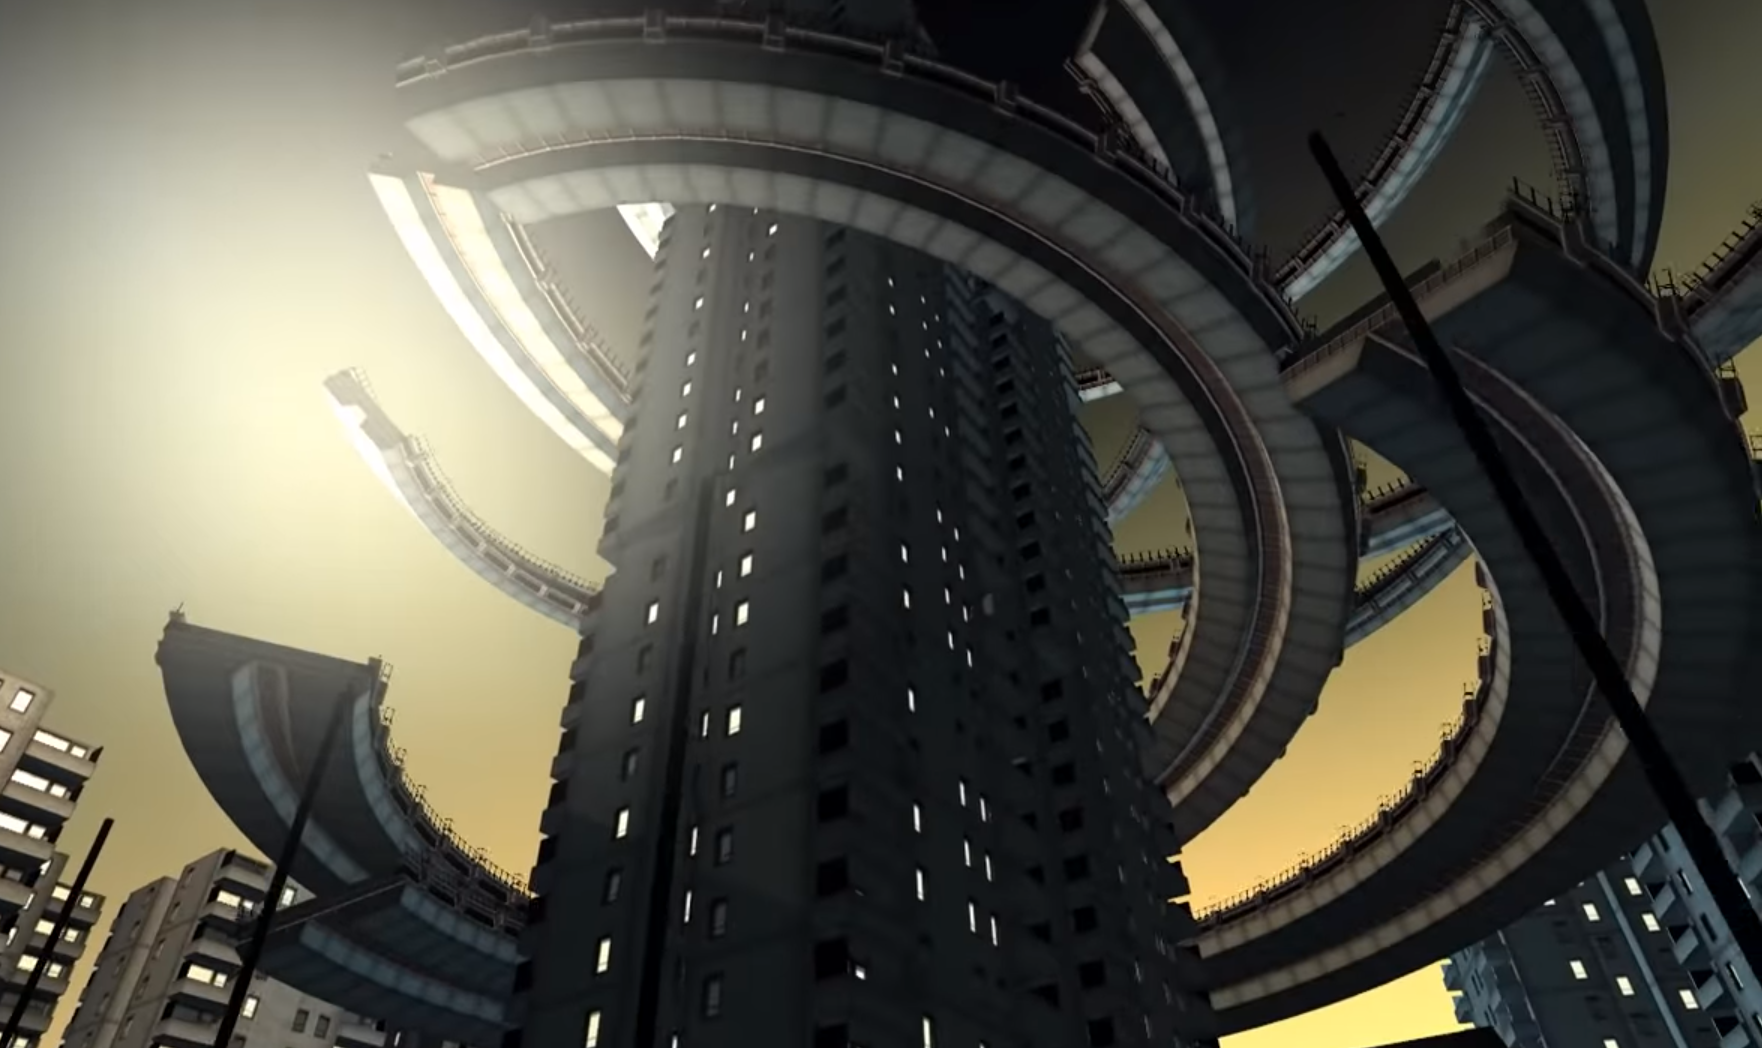
\includegraphics[width=10cm]{archivos/fr-041-debris}
	\caption{Farbrausch 41: Debris - Fuente: \href{https://www.youtube.com/watch?v=jY5Vrc5G0lk}{YouTube}}
	\label{fig:debris}
\end{figure}

Además, en el año 2004 un subgrupo dentro de Farbrausch, denominado \emph{.theprodukkt}, lanzó \emph{.kkrieger}, un juego de disparos en primera persona que ocupaba tan sólo 96kB. Este pequeño tamaño se consiguió mediante el uso de generación procedimental para las texturas y el uso de formas básicas (cubos, esferas...) combinados y deformados para los modelos. El juego [\ref{fig:kkrieger}] recibió distintos premios y fue alabado por la comunidad.\\

\begin{figure}[h]
	\centering
	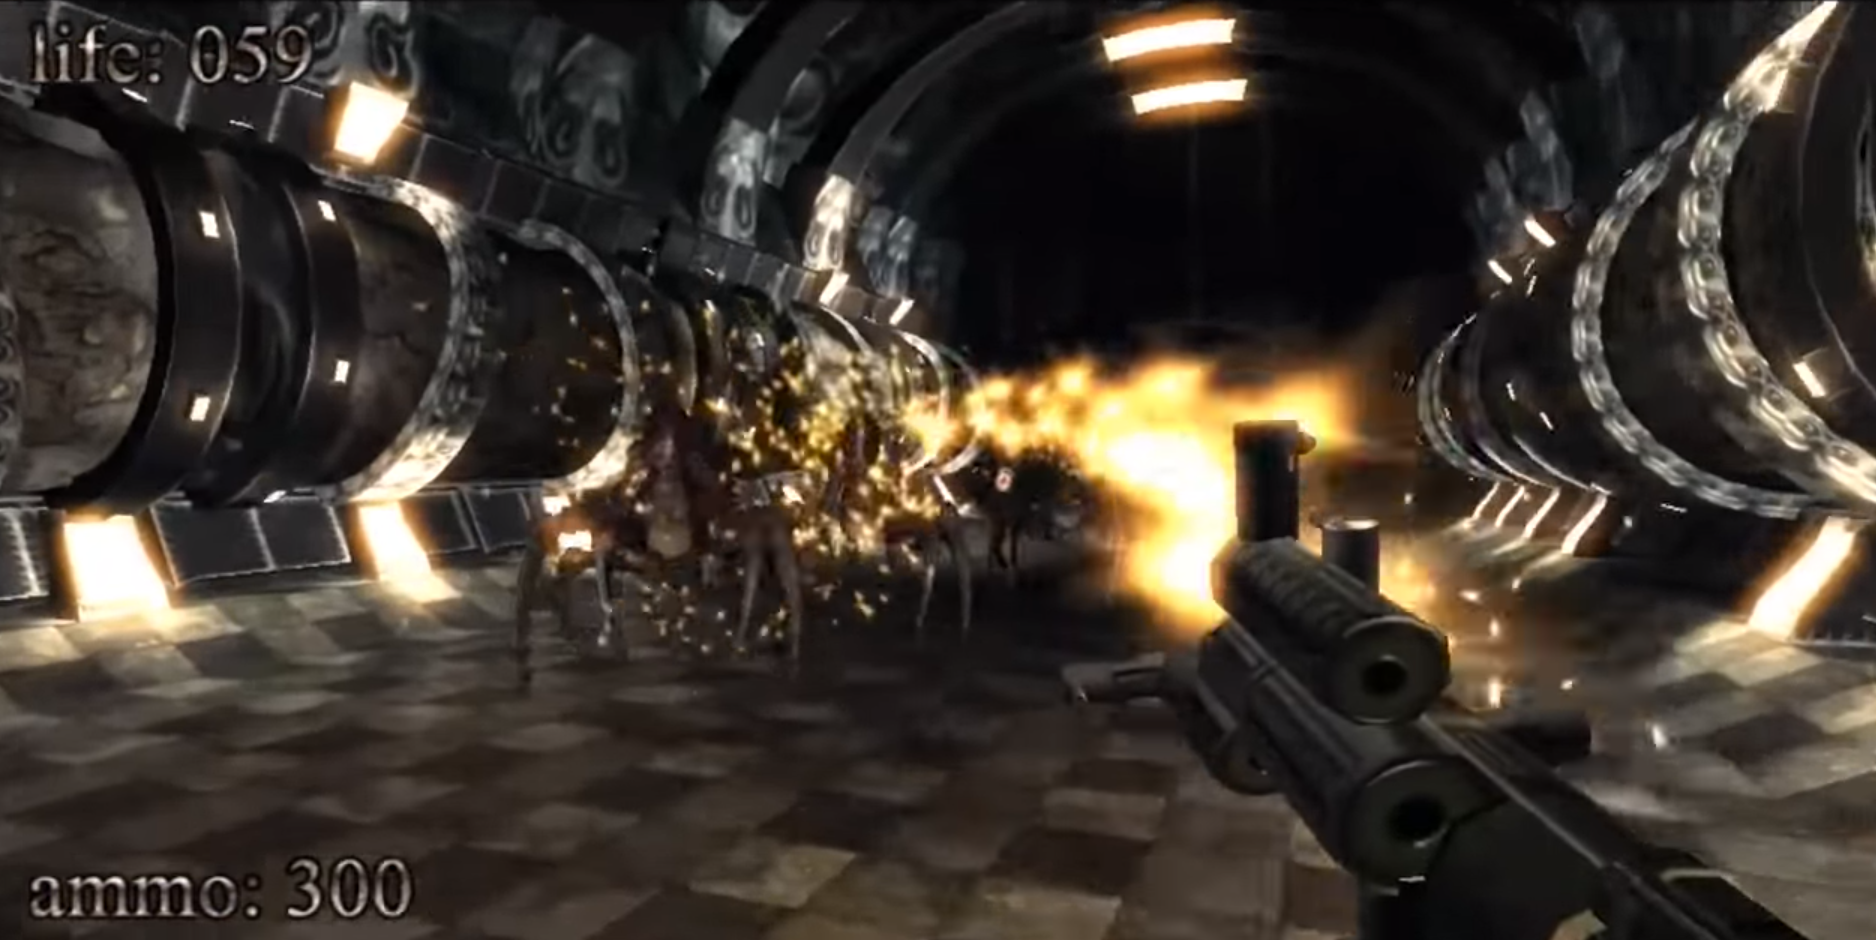
\includegraphics[width=10cm]{archivos/kkrieger}
	\caption{Videojuego de 96kB: .kkrieger - Fuente: \href{https://www.youtube.com/watch?v=2NBG-sKFaB0}{YouTube}}
	\label{fig:kkrieger}
\end{figure}

El grupo sigue en activo y siguen produciendo obras de gran calidad, contando con más de diez productos que han recibido primeros premios en distintas competiciones. En general, sus demos tienden a proseer una temática bastante urbana o robótica, con un cierto aire post-apocalíptico.
Sin embargo, su capacidad, imaginación y variedad de contenido [\ref{fig:magellan}] nunca deja de sorprender.

\begin{figure}[h]
	\centering
	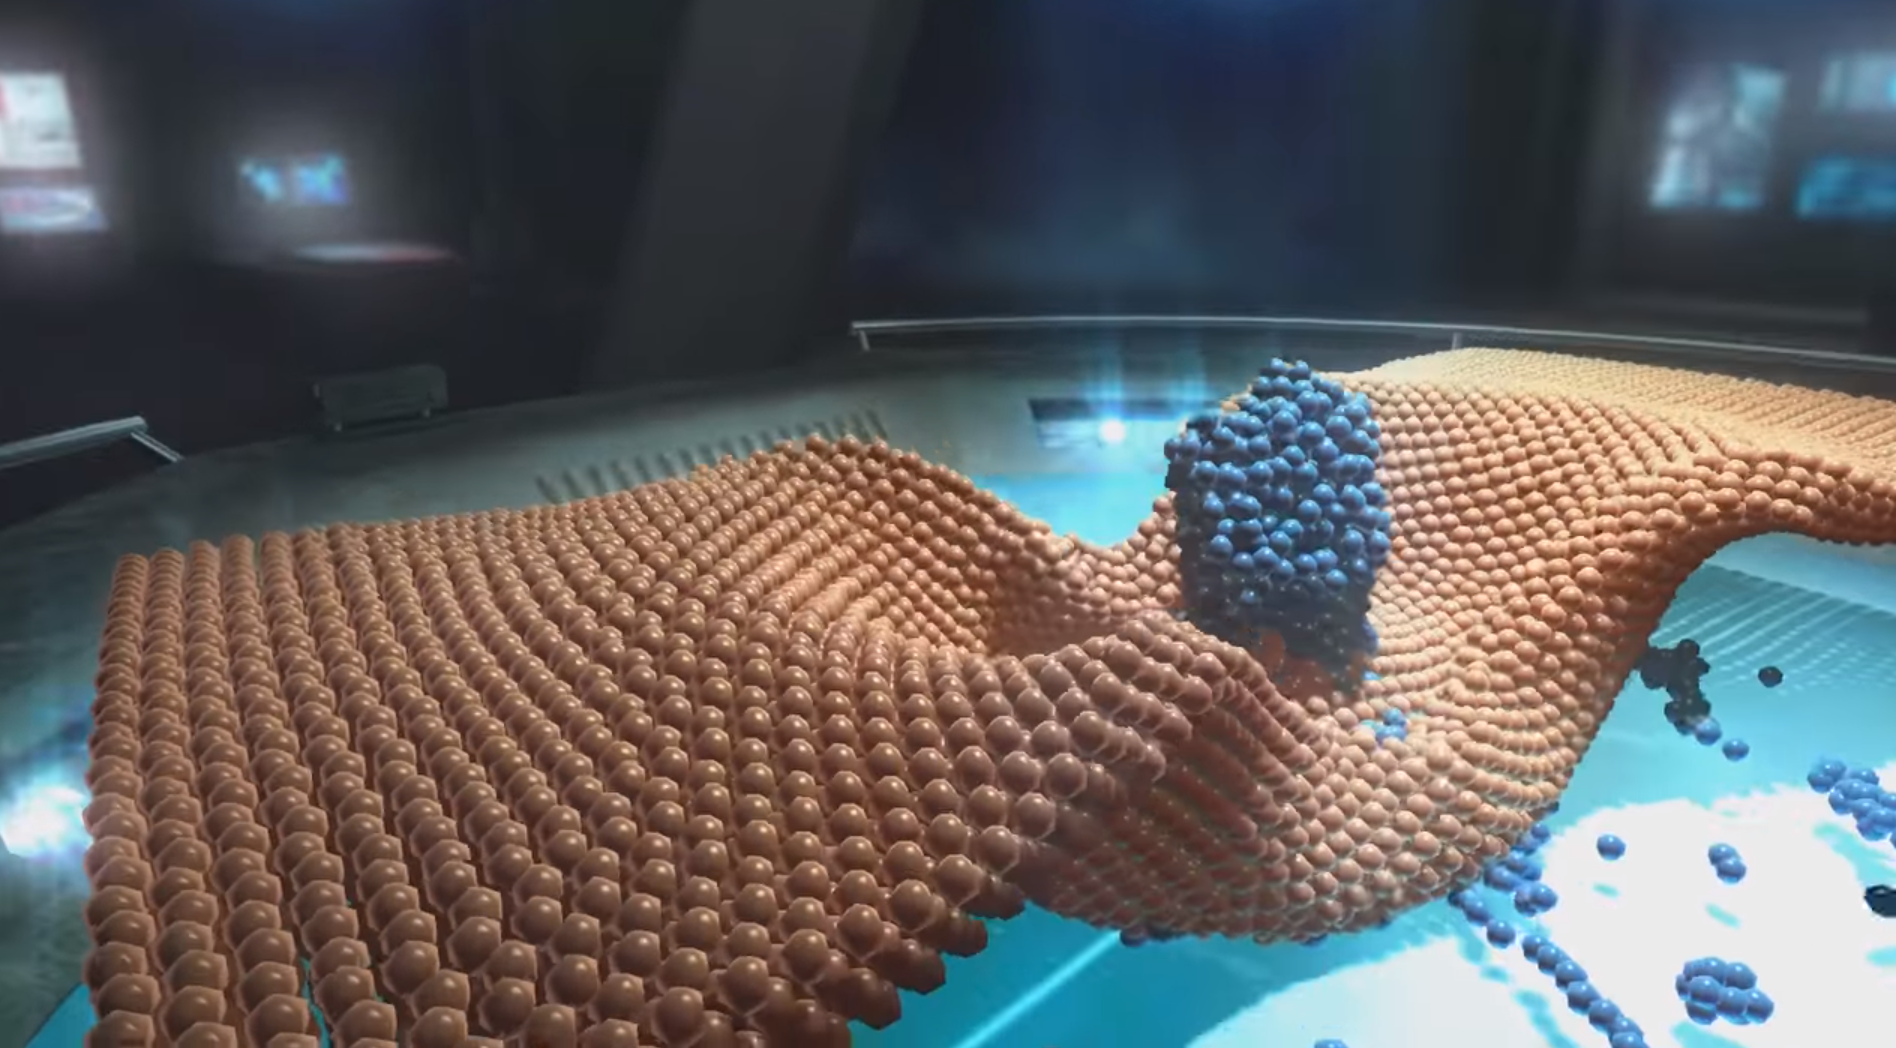
\includegraphics[width=10cm]{archivos/fr-063-magellan}
	\caption{Farbrausch 63: Magellan - Fuente: \href{https://www.youtube.com/watch?v=2Vguvli1Y0k}{YouTube}}
	\label{fig:magellan}
\end{figure}

\subsection{Future Crew}

Future Crew\footnote{\url{https://en.wikipedia.org/wiki/Future_Crew}} fue un grupo de \emph{demosceners} finés, activo principalmente entre 1987 y 1994. Su obra y legado son ampliamente conocidos en el mundo de la \emph{demoscene}. El grupo empezó creando demos para Commodore 64, aunque no tardó en pasar a PC.\\

Su trabajo es especialmente conocido no sólo por su calidad, si no también porque consiguieron resultados que en aquella época parecían imposibles. Su demo, Second Reality [\ref{fig:secondreality}], publicada en julio de 1993, se considera una de las demos más influyentes en la historia de la \emph{demoscene}. Además, el grupo fue coorganizador de la primera edición de la \emph{demoparty} Assembly.\\

\begin{figure}[h]
	\centering
	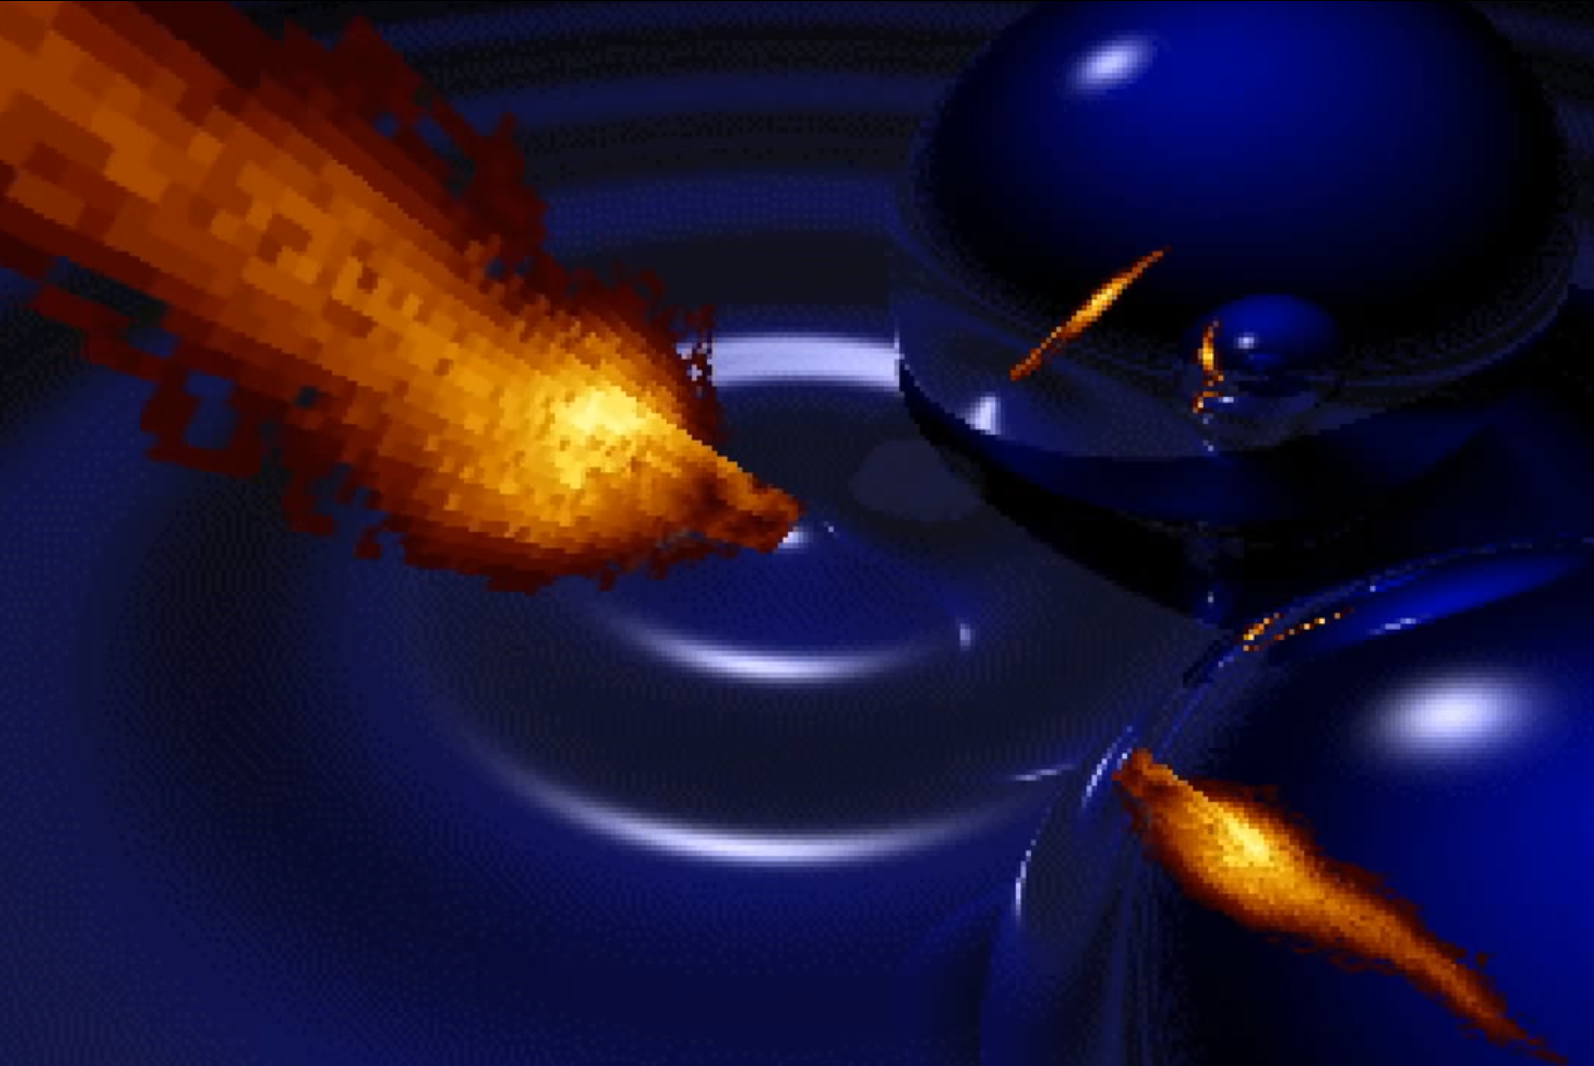
\includegraphics[width=10cm]{archivos/second-reality}
	\caption{Second Reality - Fuente: \href{https://www.youtube.com/watch?v=XezcZVu66QI}{YouTube} - En esta captura se puede ver un efecto de reflexión en dos esferas en tiempo real, mediante \emph{raytracing}}
	\label{fig:secondreality}
\end{figure}

Si bien no se produjo una disolución oficial, el grupo se fue deshaciendo paulatinamente hacia la segunda parte de los 90. La mayoría de sus miembros pasaron a la industria del videojuego o de los gráficos por computador, muchos de ellos fundando sus propios estudios, con resultados exitosos.

\subsection{PoPsY TeAm}

PoPsY TeAm\footnote{\url{http://www.popsyteam.org}} es un grupo de \emph{demosceners} franceses fundado en Lyon, en julio de 1996. Empezaron produciendo demos para Atari y posteriormente para PC.\\

Son los creadores y promotores de VIP (Very Important Party), la \emph{demoparty} más relevante de Francia. Además, PoPsY TeAm se estableció en 2001 como una asociación legalmente registrada en Francia.\\

Su demo más conocida es VIP2 [\ref{fig:vip2}], una demo que presentaron en la \emph{demoparty} holandesa TakeOver en el 2000, resultando ganadora. El objetivo de esta demo era también el de promover su propia \emph{demoparty}, VIP. Esta demo, además, fue la primera de PoPsY TeAm en usar aceleración gráfica por hardware.\\

\begin{figure}[h]
	\centering
	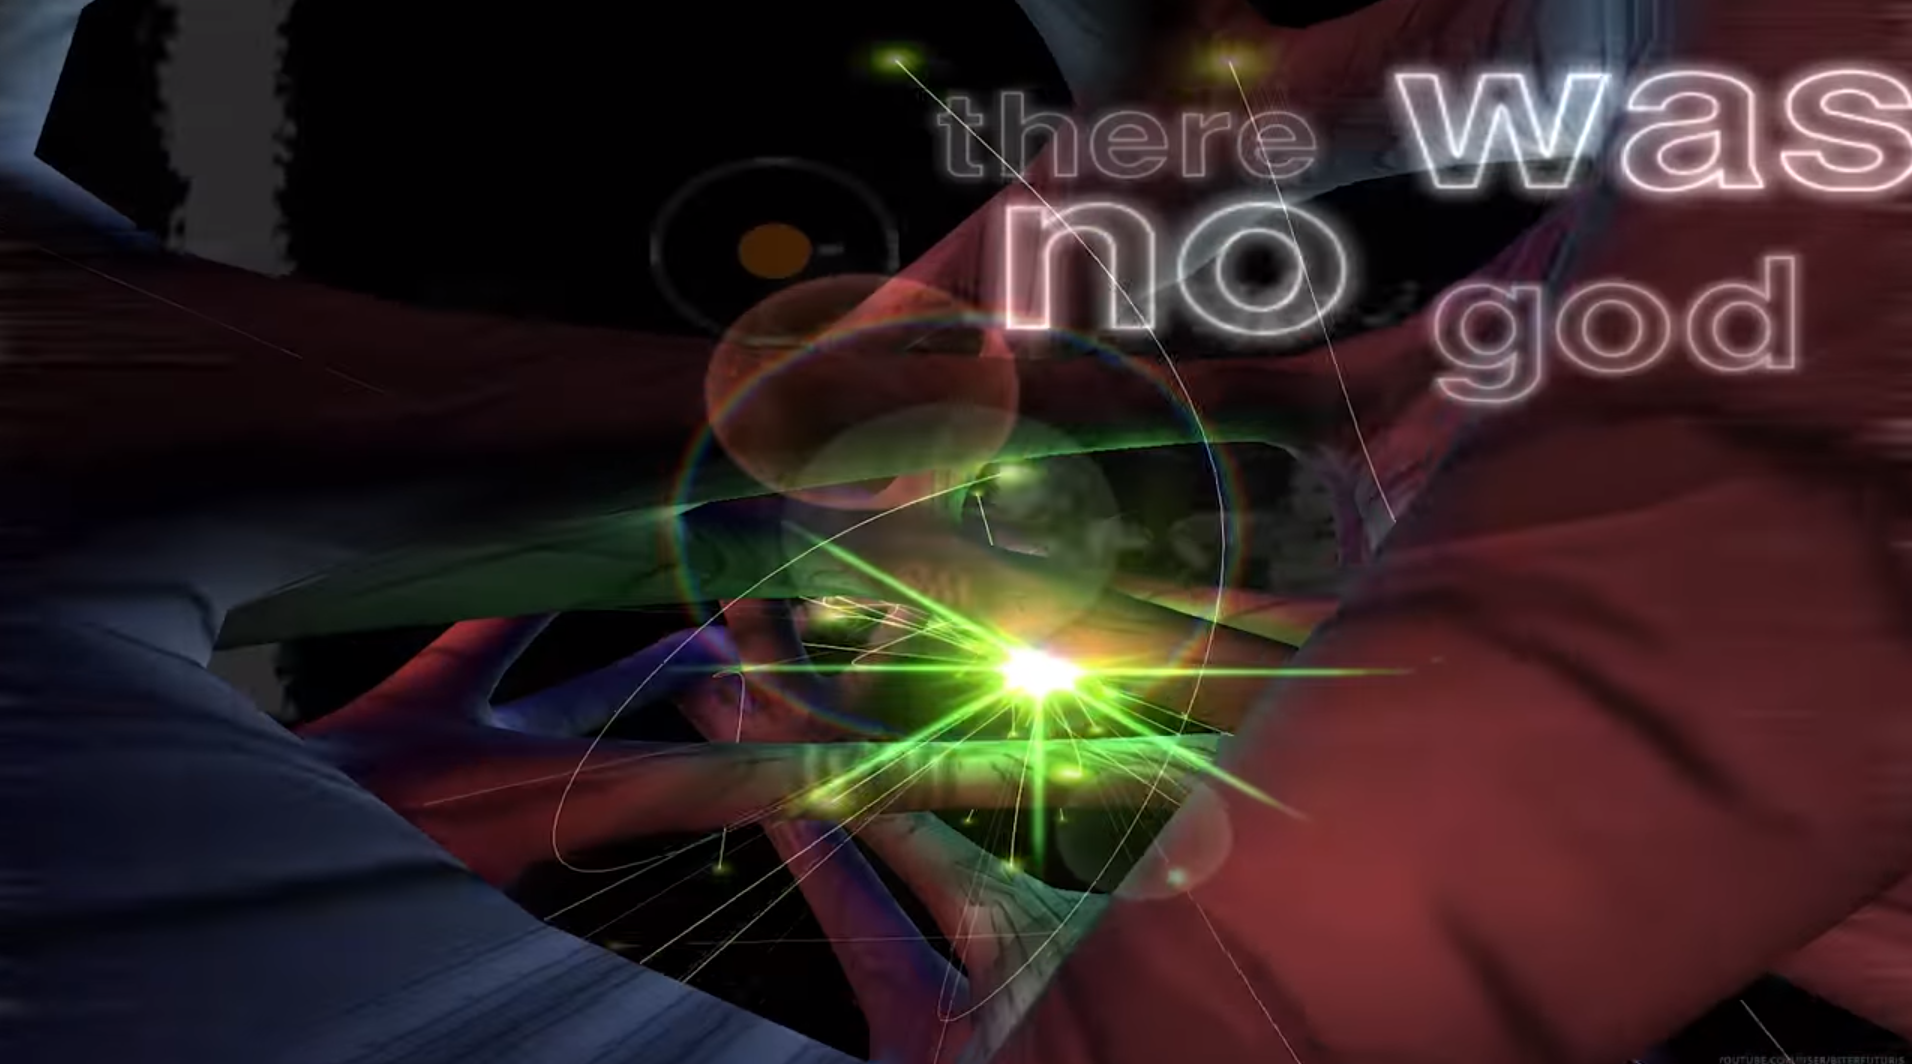
\includegraphics[width=10cm]{archivos/vip2}
	\caption{VIP2 - Fuente: \href{https://www.youtube.com/watch?v=ObtPizPFMbo}{YouTube}}
	\label{fig:vip2}
\end{figure}

El grupo siempre ha intentado promover la \emph{demoscene} y entre otras cosas, han llegado a organizar viajes en bus a diversas partes de Europa para hacer posible al resto de \emph{demosceners} de la región de Lyon atender a \emph{demoparties} europeas. Además, diversos miembros del equipo han participado en la industria del videojuego.

\subsection{Equinox}

Equinox\footnote{\url{https://equinox.planet-d.net}} es un grupo de \emph{demosceners} francés que estuvo principalmente activo entre 1988 y 2007, siendo principalmente conocido por sus demos para Atari ST, aunque sus últimas demos, publicadas pasado el cambio de milenio, fueron lanzadas para PC.

\begin{figure}[h]
	\centering
	\begin{subfigure}[b]{0.45\textwidth}
		\centering
		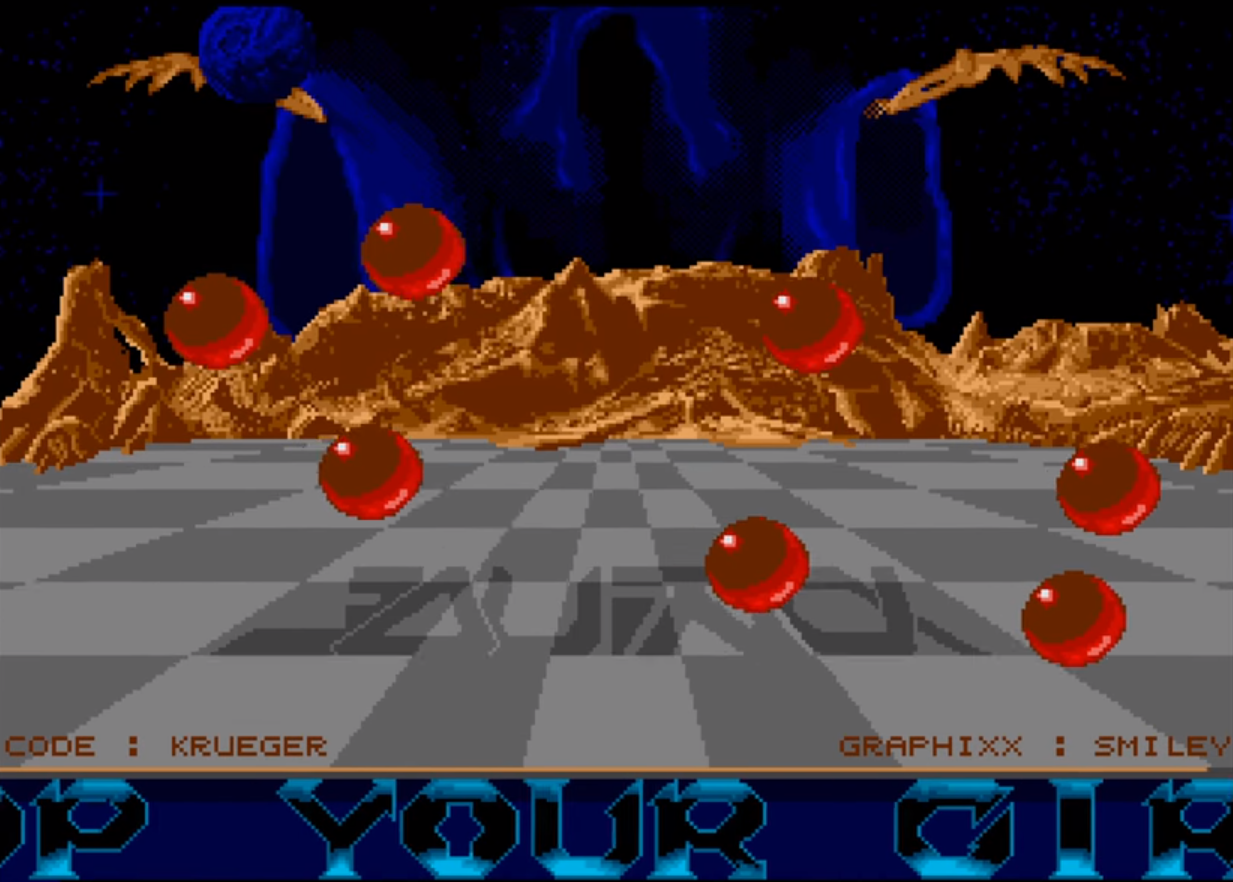
\includegraphics[width=6cm]{archivos/equinox1}
		\caption{Pupul intro (1989) - Fuente : \href{https://www.youtube.com/watch?v=efjEJIj5rhM}{YouTube}}
		\label{fig:equinox1}
	\end{subfigure}
	\begin{subfigure}[b]{0.45\textwidth}
		\centering
		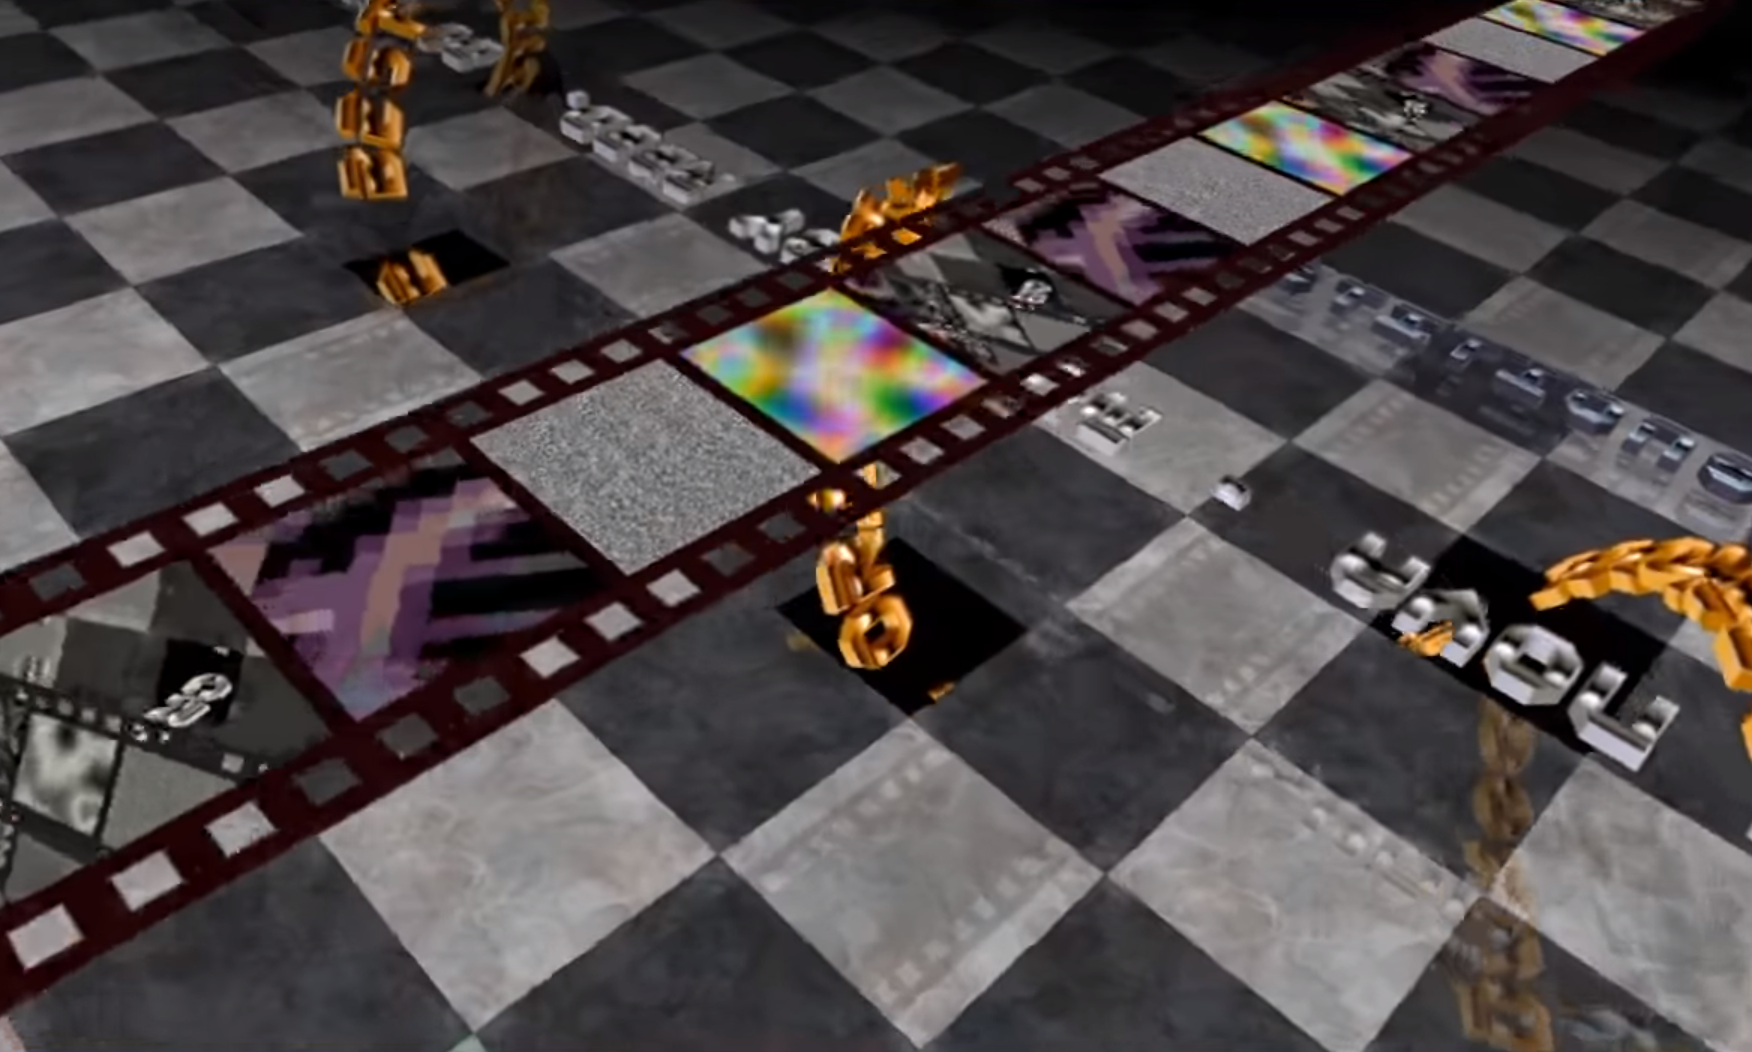
\includegraphics[width=6cm]{archivos/equinox2}
		\caption{Sota 2004 invitation intro (64k intro) - Fuente: \href{https://www.youtube.com/watch?v=cb8i0WYDLxM}{YouTube}}
		\label{fig:equinox2}
	\end{subfigure}
	\label{hace flata}
\end{figure}

\subsection{Fairlight}

FairLight\footnote{\url{http://www.fairlight.to}} es un grupo de \emph{demosceners} de origen sueco, formado en 1987. FairLight empezó creando demos para Commodore, aunque ha creado también demos para Amiga, SNES y posteriormente en PC.\\

FairLight fue fundado en 1987 por dos \emph{crackers} suecos, ex-miembros de un grupo llamado "West Coast Crackers". De hecho, FairLight no solo se dedicaba a la \emph{demoscene}, si no también al mundo del \emph{cracking}, rompiendo juegos para su lanzamiento gratuito de forma ilegal. De hecho, llegaron a hacerse especialmente conocidos por la velocidad a la que eran capaces de lanzar juegos \emph{crackeados}\footnote{\url{https://computersweden.idg.se/2.2683/1.444716/we-might-be-old-but-were-still-the-elite}}. Tal fue su impacto que en Abril de 2004, varios miembros del grupo fueron tomados por el FBI en una operación antipiratería denominada \emph{Operation FastLink}. Más de 120 personas fueron arrestadas en esta operación, en la que se consideraba a los \emph{crackers} como una organización criminal.\\

\begin{figure}[h]
	\centering
	
\includegraphics[width=10cm]{archivos/fairlight}
	\caption{Dead Ringer (por FairLight) - Fuente: \href{https://www.youtube.com/watch?v=Mc_TR4mcJKE}{YouTube} - Demo 64k ganadora de Assembly 2006}
	\label{fig:fairlight}
\end{figure}

Este es, quizás, un grupo en el que se reflejan y mezclan los orígenes de la \emph{demoscene}, provenientes del mundo del \emph{cracking}. A pesar de todo, el grupo volvió a estar en activo a partir de octubre de 2006.

\subsection{RGBA}

RGBA\footnote{\url{http://www.rgba.org}} es un grupo español de \emph{demosceners} que estuvo activo entre 2001 y 2009. Todas sus producciones fueron lanzadas para PC, principalmente en Windows.\\

Son especialmente conocidos por su demo Elevated[\ref{fig:elevated}]. Esta demo, realizada en colaboración con TBC\footnote{\url{https://demozoo.org/groups/641/}}, es especialmente conocida y celebrada por la comunidad \emph{demoscener}, situándose como la segunda más popular en el portal \url{http://www.pouet.net}.\\

Los binarios de todas sus producciones se pueden encontrar en \href{https://github.com/reality3d/rgba-prods}{GitHub}.\\

\begin{figure}[h]
	\centering
	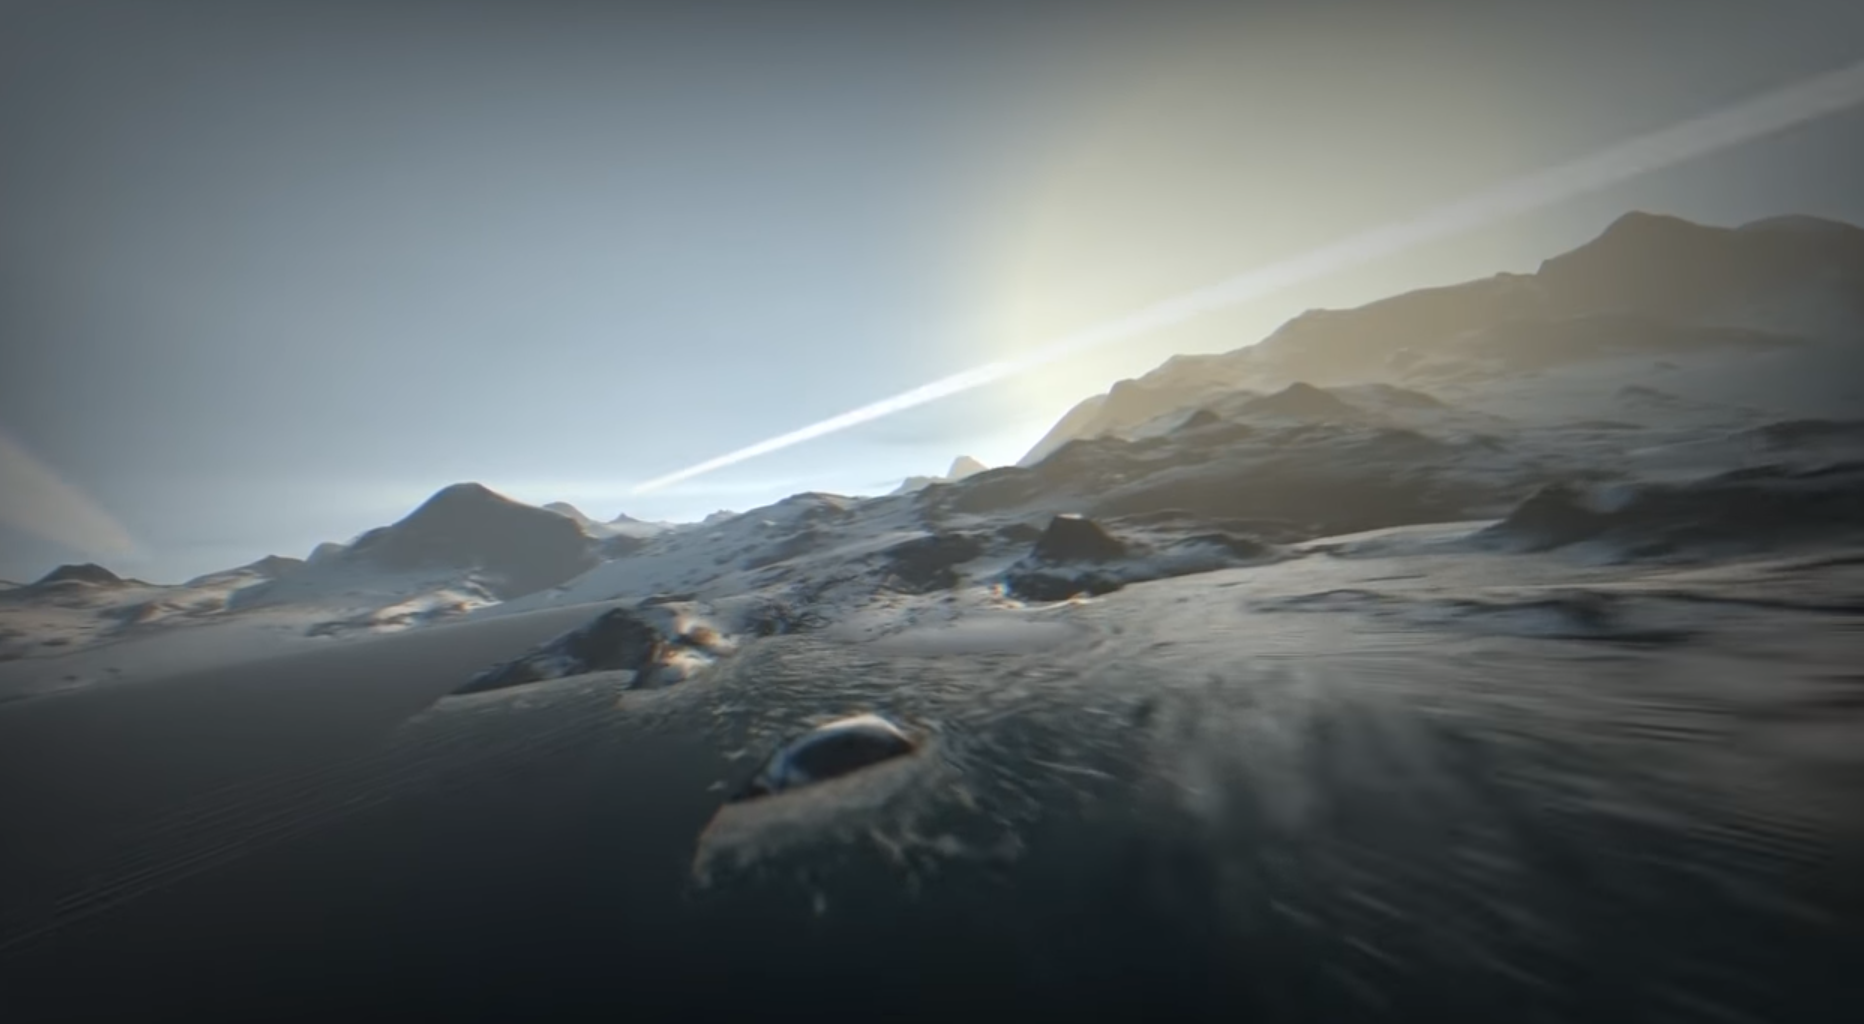
\includegraphics[width=10cm]{archivos/elevated}
	\caption{Elevated - Fuente: \href{https://www.youtube.com/watch?v=jB0vBmiTr6o}{YouTube} - Intro 4K ganadora en Breakpoint 2009}
	\label{fig:elevated}
\end{figure}

\subsection{Batman Group}

Batman Group\footnote{\url{https://demozoo.org/groups/18871/}} es un modesto grupo de \emph{demosceners} de origen español, activo desde 1993. Han producido juegos y demos para Amstrad CPC, ZX Spectrum, Amiga, Android e iOS.\\

Su demo más conocida es Batman Forever[\ref{fig:batmanforever}], para Amstrad CPC, lanzada en 2011 para la \emph{demoparty} eslovaca Forever, quedando en primera posición.\\

\begin{figure}[h]
	\centering
	
\includegraphics[width=10cm]{archivos/batmanforever}
	\caption{Batman Forever - Fuente: \href{https://www.youtube.com/watch?v=dqjZNnjNu3Y}{YouTube}}
	\label{fig:batmanforever}
\end{figure}

El grupo se vio envuelto en una polémica a finales de 2018, debido a que el grupo de desarrolladores retro \emph{4MHz} había usado para sus producciones código cedido por Batman Group sin su correcta atribución. La polémica se resolvió con la disolución de todo tipo de relación entre Batman Group y 4MHz\footnote{\url{http://www.amstrad.es/forum/viewtopic.php?t=5247}}.

\section{Portales de demoscening}
Hablar de pouet especificamente y luego del alguna más

\section{Demos destacables}
juntar y hablar de las principales demos en la demoscene, hacer referencia al top de pouet, incluir elevated y otras mas e intentar explicarlas

\section{Efectos gráficos más comunes}
comentar algunos de los efectos de la demoscene más comunes y cómo se conseguían (comentar cómo se conseguían sólo por encima)

%http://www.farbrausch.de/index.py https://en.wikipedia.org/wiki/Farbrausch
%https://en.wikipedia.org/wiki/Future_Crew https://demozoo.org/groups/357/
%http://www.popsyteam.org https://en.wikipedia.org/wiki/Very_Important_Party
%https://en.wikipedia.org/wiki/Equinox_(Atari_demogroup) https://equinox.planet-d.net/atari.html
%https://demozoo.org/groups/18871/
%https://en.wikipedia.org/wiki/Fairlight_(group)

\section{Influencia de la demoscene en la industria}

La \emph{demoscene} siempre se ha mantenido de forma discreta. Algunas de las razones de que esto sea así se han listado anteriormente, como el hecho de que hace una gran cantidad de conocimiento y pasión para poder participar de forma activa en ella. Sin embargo, esto no ha impedido dejar su huella en la industria informática, especialmente en la del videojuego.\\

La lista de personalidades que vienen del mundo de la \emph{demoscene} o se han visto influidos por ella es extensa\footnote{\url{https://chipflip.wordpress.com/2015/06/12/famous-people-who-came-from-the-demoscene/}}. A continuación se listan algunas de las más destacables:

\begin{itemize}
	\item \textbf{DICE}\footnote{\url{http://www.dice.se}}: La compañía \emph{Digital Illusions}, conocida por juegos como varios de los títulos de la saga \emph{Battefield} o \emph{Mirror's Edge Catalyst}, cuenta con una gran plantilla proveniente de la \emph{demoscene}, entre los que podemos contar miembros de FairLight.
	\item \textbf{Remedy}\footnote{\url{https://www.remedygames.com/}}: Esta compañía es especialmente conocida por la saga Max Payne. Fue cofundada por dos miembros de Future Crew. Además, esta compañía mantenía una estrecha relación con Futuremark, creadores de 3DMark, un software de pruebas de rendimiento (\emph{benchmarks}). Esta última compañía también poseía una gran cantidad de miembros provenientes de la \emph{demoscene}, contando con varios de Future Crew.
	\item \textbf{Starbreeze, Ascaron, 49Games, Techland, Lionhead Studios, Guerrilla Games}: Todas estas compañías también cuentan o han contado con miembros de la \emph{demoscene}.
	\item Will Wright, creador del vieojuego Spore, afirma que la \emph{demoscene} fue una gran influencia para al juego, debido a que este está fundamentalmente basado en la generación procedimental de contenido\footnote{\url{http://www.gamespy.com/articles/595/595975p1.html}}.
	\item John Carmack, \emph{lead programmer} de videojuegos como Wolfestein 3D, Doom y Quake, afirmó en la QuakeCon de 2011 que tiene en alta consideración a aquellos programadores que desarrollan demos de 64K, pues tienen que hacer frente a grandes limitaciones y se obtiene mucho conocimiento en el proceso\footnote{\url{https://www.youtube.com/watch?v=4zgYG-_ha28\#t=4827s}}.
	\item Jaakko Iisalo, principal diseñador de Angry Birds, fue un \emph{demoscener} activo y reconocido durante los 90.
\end{itemize}

Además, hay algunas otras subculturas informáticas que están estrechamente relacionadas con la \emph{demoscene} o derivan de la misma, como por ejemplo la música por \emph{tracker} (hay toda una comunidad de músicos que crean producciones a través del uso de \emph{trackers}, software para la producción de música).

%Importantes para la historia:
%http://widerscreen.fi/assets/reunanen-wider-1-2-2014.pdf
%http://www.oldskool.org/demos/explained/demo_history.html
%https://web.archive.org/web/20170726063815/http://tomaes.32x.de/text/faq.php#2.3.

%Elevated y otras demos por el estilo

%https://web.archive.org/web/20170726063815/http://tomaes.32x.de/text/faq.php
%http://www.oldskool.org/demos/explained/demo_history.html

%http://www.oldskool.org/demos/explained/demo_reference.html

%http://www.demoscene.info
%http://www.pouet.net/index.php
%https://en.wikipedia.org/wiki/Assembly_(demoparty)
%https://en.wikipedia.org/wiki/Demoscene

%http://widerscreen.fi/numerot/2014-1-2/crackers-became-us-demosceners/
%http://www.oldskool.org/demos/explained/demo_pages.html
%ftp://ftp.hornet.org/pub/demos/info/demonews/1998/demonews.150

%http://www.farbrausch.de/index.py 
%https://en.wikipedia.org/wiki/Farbrausch
%https://en.wikipedia.org/wiki/Future_Crew 
%https://demozoo.org/groups/357/
%http://www.popsyteam.org 
%https://en.wikipedia.org/wiki/Very_Important_Party
%https://en.wikipedia.org/wiki/Equinox_(Atari_demogroup) 
%https://equinox.planet-d.net/atari.html
%https://demozoo.org/groups/18871/	% Plantilla: Se muestran listas
%%%%%%%%%%%%%%%%%%%%%%%%%%%%%%%%%%%%%%%%%%%%%%%%%%%%%%%%%%%%%%%%%%%%%%%%
% Plantilla TFG/TFM
% Escuela Politécnica Superior de la Universidad de Alicante
% Realizado por: Jose Manuel Requena Plens
% Contacto: info@jmrplens.com / Telegram:@jmrplens
%%%%%%%%%%%%%%%%%%%%%%%%%%%%%%%%%%%%%%%%%%%%%%%%%%%%%%%%%%%%%%%%%%%%%%%%

\chapter{Objetivos}

Aprender el bajo nivel y rendimiento, crear varios efectos básicos, crear un efecto más complejo		% Plantilla: Se muestran tablas
%%%%%%%%%%%%%%%%%%%%%%%%%%%%%%%%%%%%%%%%%%%%%%%%%%%%%%%%%%%%%%%%%%%%%%%%
% Plantilla TFG/TFM
% Escuela Politécnica Superior de la Universidad de Alicante
% Realizado por: Jose Manuel Requena Plens
% Contacto: info@jmrplens.com / Telegram:@jmrplens
%%%%%%%%%%%%%%%%%%%%%%%%%%%%%%%%%%%%%%%%%%%%%%%%%%%%%%%%%%%%%%%%%%%%%%%%

\chapter{Metodología}

\section{Software}

\begin{itemize}
	\item \textbf{Toggle}\footnote{\url{https://toggl.com/}}: Se utilizará la herramienta online Toggl para contabilizar el tiempo dedicado a cada parte del proyecto. Esto permitirá poder analizar qué partes del trabajo han requerido más dedicación y por qué, ayudando a completar el estudio.
	\item \textbf{Git}\footnote{\url{https://git-scm.com}}: Se utilizará Git para el control de versiones. El uso de Git nos permitirá, además, tener un registro detallado de la evolución del código. El código para este proyecto se aloja en GitHub\footnote{\url{https://github.com/donluispanis/TFG}}.
	\item \textbf{Make}\footnote{\url{https://www.gnu.org/software/make/}}: El código de este proyecto será compilable tanto en las plataformas Windows como Linux. Para ello, el uso de la herramienta Make facilitará la compilación de los proyectos así como su portabilidad.
	\item \textbf{MinGW}\footnote{\url{http://www.mingw.org}}: MinGW es un entorno de desarrollo para Windows que ofrece un entorno similar al de GNU. Se usará para compilar tanto el código como las librerías en Windows, haciendo la portabilidad más consistente y sencilla.
	\item \textbf{GCC}\footnote{\url{https://gcc.gnu.org}}: GCC es una colección de compiladores con soporte para C++. Se usará para compilar el código de este proyecto, tanto en Windows (a través de MinGW) como en Linux (de forma nativa).
	\item \textbf{GLFW}\footnote{\url{https://www.glfw.org}}: GLFW es una librería multiplataforma para OpenGL que facilita los procesos de creación de ventana, generación de contexto y manejo de input. 
	\item \textbf{OpenGL}\footnote{\url{https://www.opengl.org}}: OpenGL es una extendida librería para la creación y manipulación de gráficos bidimensionales y tridimensionales. En este proyecto, sin embargo, su uso será mínimo y restringido. Se utilizará tan solo para dibujar una textura en nuestra ventana. Será mediante la manipulación de esta textura que generaremos gráficos. OpenGL, por tanto, será un mero mediador, redibujando constantemente la misma textura en pantalla.
	\item \textbf{Valgrind}\footnote{\url{http://valgrind.org}}: Valgrind es una herramienta de depuración y perfilado. Se utilizará para realizar pruebas de rendimiento y para comprobar el correcto funcionamiento del programa. 
	\item \textbf{Compiler Explorer}\footnote{\url{https://godbolt.org}}: Compiler Explorer es una herramienta online que permite ver la salida en ensamblador del código escrito de forma instantánea. Resultará muy útil para analizar y entender mejor el código que se ejecuta.
\end{itemize}

\section{Tests de rendimiento}

Se pretende recopilar una serie de resultados cuantificables que muestren el coste de distintos tipos de operaciones computacionales, tanto a nivel de coste temporal como espacial (y cantidad de instrucciones).\\

Se realizará un análisis exhaustivo de los resultados obtenidos, exponiéndolos y razonando acerca de los mismos.\\

Para realizar estas pruebas, se procederá a la ejecución de pequeños programas que contengan pruebas concretas. Las pruebas que se propone realizar son: operaciones matemáticas con números enteros, operaciones matemáticas con números en coma flotante, coste de la reserva y liberación de memoria, coste del acceso a memoria y coste de los bucles y las operaciones condicionales.\\

Tras analizar los resultados, se elaborarán una serie de directrices para escribir código que sea generalmente más rápido y/o más fácilmente optimizable por el compilador. Para poder analizar correctamente los resultados obtenidos, se tendrá en cuenta el código ensamblador generado por el compilador.\\

\section{Entorno: motor gráfico}

El objetivo final de este proyecto es recopilar e implementar una serie de efectos gráficos. Sin embargo, para poder realizar esta tarea, es necesario disponer de un entorno que nos permita realizar labores básicas, como gestión de la ventana o de input.\\

Mediante la creación de un entorno se asegura un flujo de trabajo consistente entre todas las demos, así como la reutilización de código. Será necesaria, por tanto, la creación de un motor gráfico. Este motor deberá de ser lo más sencillo posible, pues debe limitarse a facilitar tareas básicas, pero no debe ofrecer soluciones a problemas complejos o específicos a una demo. Este motor debe ser conciso y ligero, pues debe influir lo mínimo posible en el rendimiento de la demo.\\

Este motor debe darnos soporte para: manejo de la ventana, acceso a un espacio de memoria donde sea posible manipular gráficos, manejo de entradas de teclado, dibujado básico en ventana (puntos, líneas, areas rectangulares y texto)

\section{Las demos}

Para afrontar cada una de las demos, se seguirá un procedimiento común que se expone a continuación.

\subsection{Búsqueda de información}

En una primera fase, se procederá a la búsqueda de documentación e información sobre la demo. Esto incluye tanto vídeos como imágenes, además de tutoriales o explicaciones teóricas. En esta fase, se plantea recopilar tanta información acerca de la demo como sea posible, y lograr un modelo teórico básico acerca de cómo debería funcionar.

\subsection{Planteamiento formal}

Una vez se ha recopilado información sobre la demo a estudio y se posee un conocimiento suficiente sobre la misma, se procede a un planteamiento formal, previo a su implementación. Este planteamiento incluye entender en profundidad la base matemática de la demo, si la hay. Se debe realizar un análisis y explorar distintos puntos de vista desde los que se podría implementar la demo.

\subsection{Implementación}

Analizada la demo, y se habiendo razonado sobre el mejor modo de desarrollarla, se procede a la fase de implementación en código de la demo. Esta es una fase experimental y que permite flexibilidad. Es posible que sea necesario probar distintos acercamientos, buscando el que más se adecúe al resultado que se busca y que ha sido definido en el planteamiento formal de la demo.

\subsection{Refinamiento}

Cuando la demo ya está completada a nivel de funcionalidad, se procede a su refinamiento y refactorización. En esta fase se busca hacer el código más legible (nombres de variables y funciones explícitos, correcta documentación del código...) así como hacer el código más eficiente (identificar los factores críticos del programa y buscar e implementar soluciones más eficientes).	% Plantilla: Se muestran figuras
%%%%%%%%%%%%%%%%%%%%%%%%%%%%%%%%%%%%%%%%%%%%%%%%%%%%%%%%%%%%%%%%%%%%%%%%
% Plantilla TFG/TFM
% Escuela Politécnica Superior de la Universidad de Alicante
% Realizado por: Jose Manuel Requena Plens
% Contacto: info@jmrplens.com / Telegram:@jmrplens
%%%%%%%%%%%%%%%%%%%%%%%%%%%%%%%%%%%%%%%%%%%%%%%%%%%%%%%%%%%%%%%%%%%%%%%%

\chapter{Tests de rendimiento}

\section{Implementación}
\section{Resultados}

\chapter{El motor gráfico}

Antes siquiera de poder empezar a desarrollar la primera demo, es necesario crear un entorno que sea capaz de automatizar las tareas más básicas que no son competencia directa de la demo, como por ejemplo gestión de la ventana y de las entradas de teclado. Este código será común y necesario a todas las demos, pues independientemente de sus características concretas, todas ellas necesitarán una ventana y un espacio en el que poder volcar datos.\\

Es por ello que antes de empezar con la primera demo, se hizo necesario el desarrollo de un pequeño \emph{framework} que permitiese gestionar de la forma más rápida y sencilla posible aquellas tareas que no debían ser responsabilidad directa de la demo. 

\section{Investigación inicial}

Una de las principales influencias en el desarrollo de la versión inicial del motor gráfico fue OneLoneCoder\footnote{\url{https://www.youtube.com/channel/UC-yuWVUplUJZvieEligKBkA}}. Este programador británico tiene una colección de tutoriales con alto valor educativo y en muchos de ellos explica incluso técnicas de programación de la vieja escuela. Fue a raíz de visualizar estos vídeos donde vi expuestos muchos de los problemas a los que me tendría que enfrentar en el futuro.\\

El ejemplo más claro: en sus primeros vídeos, este programador siempre repite el mismo código para poner en marcha una consola usable, hasta que decide crear un modelo básico que le permita reutilizar este código.\\

Este canal ha tenido un gran valor formativo para mí, ya que me permitió identificar una serie de problemas que de otro modo sólo hubieran aparecido en un momento más avanzado del desarrollo, y que sin embargo, hubieran resultado costosos de solventar.\\

Inicialmente, estos fueron los objetivos que pretendía cubrir el motor gráfico:
\begin{itemize}
	\item \textbf{Reutilización de código}: tareas como abrir y cerrar la ventana o gestionar el dibujado son necesarias en absolutamente todas las demos, por lo que todo código relacionado con la ventana y/o el dibujado debería poder ser reutilizado sin tener que duplicarse.
	\item \textbf{Encapsulación de toda lógica no relacionada con la demo}: uno de los principales objetivos que se persiguen con la creación de un motor gráfico es la claridad. La implementación de una demo \textbf{sólo debe contener lógica que está directamente relacionada con sus detalles de implementación}, es decir, con los algoritmos o técnicas de los que la demo hace uso. De este modo, el código de una demo sólo refleja la lógica de la misma, sin exponer la lógica necesaria para la de gestión de ventana, que no es responsabilidad de la misma. Esto permite un código más claro y conciso, más fácil de implementar, usar, refinar y entender.
		\begin{itemize}
			\item \textbf{Encapsulación de la ventana}: una demo no debe ser consciente de qué es necesario para crear o borrar una ventana, todo lo que debe hacer es ser poder decir "quiero crear una ventana" o "quiero cerrar la ventana" pero no debe ocuparse de los detalles de implementación.
			\item \textbf{Encapsulación del dibujado}: una demo no debe tener responsabilidad de gestionar el dibujado en ventana. Todo lo que una demo necesita saber es en qué lugar de memoria debe escribir para que esos datos sean dibujados en pantalla, pero no debe encargarse de la gestión del dibujado.
		\end{itemize}
	\item \textbf{Abstracción de la plataforma}: el código de una demo no debe contener detalles de implementación relativos a la plataforma en que se ejecuta. Desde el punto de vista de la demo, todo lo que importa es el algoritmo, y este debe ser el mismo independientemente del sistema operativo y del \emph{hardware} sobre el que se ejecuta.
\end{itemize}

Durante el desarrollo, no obstante, nuevas necesidades se irían añadiendo, ya fuera por nuevas decisiones de diseño, refinamiento de código o por nuevas necesidades de las demos:
\begin{itemize}
	\item \textbf{Abstracción de las librerías y tecnologías utilizadas}: tras varias iteraciones sobre el desarrollo inicial, fue necesario un refinamiento. El motor gráfico contenía demasiada lógica, y era lógica acoplada a la gestión de la ventana o del dibujado. Esto levantó una pregunta: ¿y si en algún momento necesito cambiar las librerías que utilizo o incluso prescindir de las mismas? Esta era una posibilidad bastante probable, dado que a lo largo del desarrollo de un proyecto y conforme surgen nuevas necesidades, puede que las tecnologías elegidas inicialmente no satisfagan las condiciones actuales. Por tanto, el motor gráfico no debía estar acoplado a las tecnologías que usaba, si no que debía mediar con ellas mediante el uso de interfaces.
	\item \textbf{Abstracción de los eventos de teclado}: conforme el desarrollo avanzó, se hizo aparente que en muchas ocasiones era útil permitir al usuario modificar parámetros de la demo en tiempo real, en cierto modo permitir "jugar" con la demo. Era necesario por tanto permitir el manejo de eventos de teclado, aunque su uso debía estar abstraído de su implementación, de forma que desde el punto de vista de la demo, todo lo que se pudiera hacer es "quiero saber el estado de esta tecla".
	\item \textbf{Abstracción del dibujado de texto en pantalla}: una vez más, al continuar con el desarrollo, se hizo aparente la necesidad de poder dibujar texto en pantalla. El motor gráfico debía ser por tanto capaz de abstraer o enmascarar las rutinas de dibujado del texto, de modo que desde la perspectiva de la demo todo lo que importase fuera dibujar un texto con un color, posición y tamaño determinados, independientemente de la implementación.
	\item \textbf{Uso de mecanismos de dibujado seguros para formas básicas}: aunque inicialmente parecía que cualquier tipo de dibujado debía ser responsabilidad de la demo, pronto se hizo aparente que ciertas rutinas se repetían de forma constante. Además, mientras que en un inicio el dibujado de un punto o una línea era responsabilidad de la demo, pronto se vio que desde el punto de vista de la demo, estas responsabilidades no tienen interés, ya que la capacidad de poder dibujar una línea es importante, pero no cómo se dibuja. 
		\begin{itemize}
			\item \textbf{Dibujado de puntos}: desde la perspectiva de una demo, tan sólo importan la posición, color y tamaño de un punto que se quiera dibujar en pantalla. La gestión de si ese punto está dentro o fuera de los límites de pantalla o la gestión del tamaño del punto no debería ser competencia de la demo, si no del motor.
			\item \textbf{Dibujado de líneas}: una demo debe ser capaz de solicitar el dibujado de una línea dados dos puntos, un color y un tamaño, pero no debe responsabilizarse de la gestión de los límites en pantalla ni del algoritmo de dibujado para una línea.
			\item \textbf{Dibujado de rectángulos}: una demo debe ser capaz de dibujar rectángulos en pantalla, especialmente útiles para el borrado de la pantalla o de regiones de la misma, pero no debe conocer sus detalles de implementación.
		\end{itemize}
\end{itemize}

Con todos estos puntos en mente, y de forma progresiva, se fue desarrollando, revisando y refinando la creación de un motor gráfico que sirviera como marco de trabajo efectivo para el desarrollo de una demo.

\section{Características}

%@startuml
%
%abstract ClassicDemoTemplate {
%  .. Public methods ..
%  +Construct(name, width, height, fullscreen)
%  +Run()
%  +Close()
%  .. Methods usable by children ..
%  #GetWindowManager()
%  #RenderDot(position, colour, size)
%  #RenderLine(position, colour, size)
%  #ClearScreen(square, colour)
%  #IsPixelOutOfBounds(position)
%  .. Pure virtual methods overriden by children ..
%  -Init()
%  -Update(deltaTime)
%  -Destroy()
%}
%
%interface IWindowManager {
%  +CreateWindow(name, width, height, fullscreen)
%  +UpdateWindow()
%  +DestroyWindow()
%}
%
%interface IRenderManager {
%  +InitialiseRender(width, height)
%  +DrawToScreen()
%  +DisposeRender()
%}
%
%class OpenGLRenderManager {
%}
%
%class GLFWWindowManager {
%}
%
%OpenGLRenderManager -|> IRenderManager
%GLFWWindowManager --|> IWindowManager
%
%IRenderManager -* GLFWWindowManager
%ClassicDemoTemplate *- IWindowManager
%
%hide empty members
%
%@enduml

\begin{figure}[h]
	\centering
	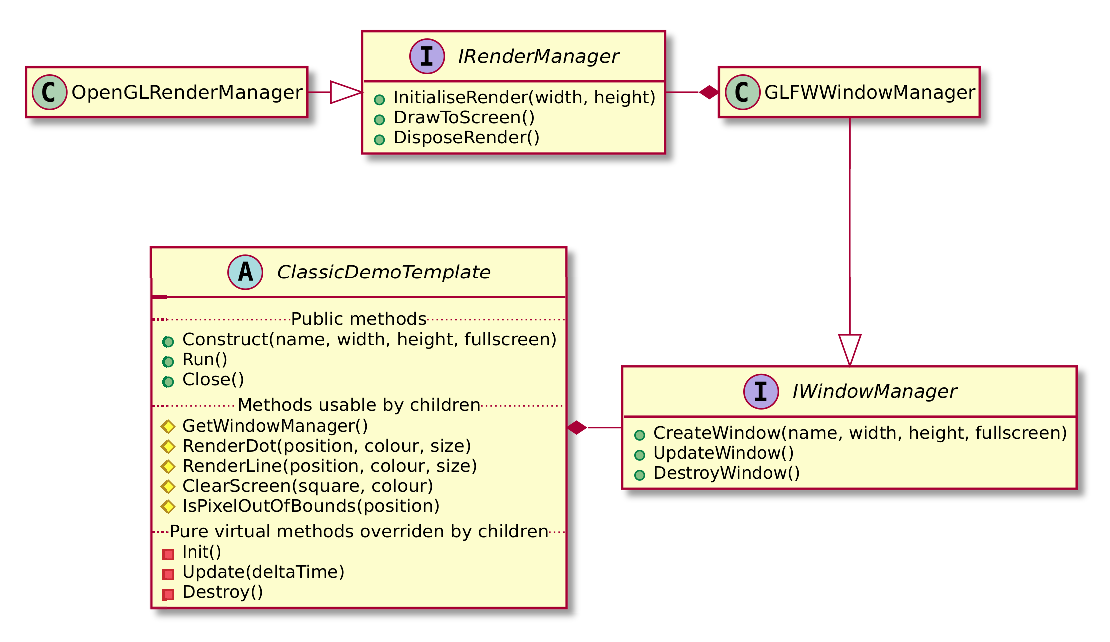
\includegraphics[width=15cm]{archivos/classicdemotemplateuml}
	\caption{Diagrama simplificado de la estructura del motor gráfico}
	\label{fig:classicdemotemplateuml}
\end{figure}

La figura [\ref{fig:classicdemotemplateuml}] presenta la estructura simplificada del motor gráfico.\\

Como se puede observar, el motor (\emph{ClassicDemoTemplate)} delega las tareas de gestión de la ventana en una interfaz cuyos métodos más relevantes permiten crear, actualizar y destruir la ventana. De este modo, el motor gráfico está completamente desacoplado de las tareas concretas de gestión de la ventana.\\

La implementación concreta de la interfaz (\emph{GLFWWindowManager}) utiliza, como su nombre indica, la librería GLFW para gestionar la ventana. Esta es una librería de código abierto y multiplataforma que hace más sencilla la gestión. No obstante, la implementación concreta está completamente desacoplada del sistema, por lo que si fuera necesario migrar a una tecnología distinta (como SDL, SFML o accediendo directamente a la API gráfica de Windows (WinAPI) o Linux (X11)), se podría hacer siempre y cuando esta nueva clase implementase la interfaz definida.\\

A su vez, \emph{GLFWWindowManager} hace uso de la interfaz \emph{IRenderManager}, que implementa \emph{OpenGLRenderManager}. Esto permite, una vez más, cambiar la tecnología de dibujado sin tener que cambiar necesariamente el sistema de ventanas. De este modo también se separa de forma efectiva todo el código relativo a la gestión de la ventana con respecto al código relativo al dibujado, lo que facilita la claridad y mantenimiento del código.\\

En nuestro caso, el dibujado se hace mediante OpenGL, una especificación para gráficos 3D multiplataforma. No obstante, OpenGL es utilizado como un mero mediador, cuyo único uso es el dibujado de una textura en pantalla. Es esta textura que se \emph{renderiza} de forma cíclica a la que el usuario tiene acceso y puede modificar, dibujando así en pantalla.\\

De este modo, la clase principal de nuestro motor \emph{(ClassicDemoTemplate)} no tiene responsabilidad directa sobre la gestión de la ventana y el dibujado, de modo que aunque las librerías o tecnologías utilizadas cambiasen, toda la lógica contenida en el motor seguiría siendo usable.\\

Como se puede observar en el diagrama, esta clase principal es una clase abstracta, lo que implica que debe ser implementada por una clase concreta para poder instanciarse. Toda demo que use este motor gráfico debe heredar de \emph{ClassicDemoTemplate}. Esto permite definir una estructura que todas nuestras demos deberán satisfacer para hacer un uso efectivo de nuestro motor.\\

En primer lugar, se exponen únicamente tres métodos, \emph{Construct}, \emph{Run} y \emph{Close}. Esto implica que cualquier demo ha de ser completamente usable mediante estos tres métodos.\\

A continuación, \emph{ClassicDemoTemplate} expone una serie de métodos que pueden ser utilizados únicamente por las demos, que heredan de esta clase. Estos métodos aportan funcionalidad común que resultan útiles en la mayor parte de las demos, como dibujar puntos y líneas o comprobar si un píxel determinado está dentro de los límites de la ventana.\\

Por último, hay tres métodos virtuales y privados que toda demo debe implementar: \emph{Init}, \emph{Update} y \emph{Destroy}. La llamada a estos método es gestionada por \emph{ClassicDemoTemplate}, por lo que el usuario tan sólo debe preocuparse de implementarlos. Los métodos \emph{Init} y \emph{Destroy} permiten inicializar y destruir las variables los datos propios de la demo. El método \emph{Update} es llamado en el bucle de ejecución del programa y recibe el tiempo sucedido desde el último fotograma. Este método contendrá toda la lógica necesaria para actualizar los datos que maneja nuestro programa a lo largo del tiempo. 

\subsection{La textura de dibujado y el píxel}

\subsection{Detectar input}

Por básica que pueda parecer la detección de entradas de teclado, esta característica no fue implementada hasta un estado relativamente avanzado del desarrollo del proyecto. Aunque esto pueda resultar difícil de entender desde el punto de vista del usuario, desde el punto de vista del desarrollador, las entradas de teclado sirven principalmente para "jugar" con la demo y para ajustar valores, es decir, que resultan útiles en el proceso de refinamiento de la demo, pero son irrelevantes en el proceso de creación de la misma. Es por ello que disponer de \emph{input} para las demos no es algo que se priorizara, ya que estaba mucho más interesado en el desarrollo de los algoritmos y métodos necesarios para cada demo que no en poder "jugar" con los resultados.\\

No obstante, llegó un punto en el desarrollo en el que las demos, además de ser funcionales, debían ser manipulables, modificables de forma dinámica, y fue en este momento cuándo se planteó la pregunta de cómo gestionar las entradas de teclado.\\

Las entradas de teclado se gestionan desde la ventana, por lo que tenía claro que su gestión debería ser parte de la responsabilidad de \emph{GLFWWindowManager}. Era importante, sin embargo, saber en qué eventos de teclado estaba interesado.\\

Estos eran los eventos que me interesaban: saber el momento en que la tecla se pulsa por primera vez, saber el momento en el que la tecla se suelta y saber si la tecla se está manteniendo pulsada o no. Sin embargo, GLFW sólo daba acceso directo a saber si la tecla estaba pulsada o no, por lo que la lógica para el resto de eventos debía ser implementada por mi parte.\\

GLFW permitía otra opción, además, en lugar de preguntar por el estado de una tecla concreta, es posible pasarle un método delegado que sea llamado cada vez que se produce un evento, de forma que este método sobre el que nosotros tenemos control pueda gestionar los eventos en los que estamos interesados. Por razones de simplicidad y mantenibilidad, decidí optar sin embargo por la opción de preguntar por el estado de las teclas.\\

Esta opción sin embargo planteaba un problema de eficiencia: la única forma de saber si una tecla cualquiera está pulsada o no es almacenando y actualizando el estado de todas las teclas. Esto implicaría tener que estar actualizando el estado de más de 100 teclas cuando tan sólo tenemos interés en unas pocas. Y precisamente lo que decidí fue añadir un método que permitiera registrar interés en una tecla. Esto hace que la gestión de \emph{input} en una demo sea ligeramente más compleja (para poder preguntar por el estado de una tecla, esta debe haberse registrado previamente). Sin embargo, a cambio de esta ligera complejidad añadida, hay una gran ganancia en rendimiento, ya que en lugar de actualizar el estado de \emph{todas} las teclas del teclado por fotograma, sólo actualizaremos el estado de aquellas que nos interesan, y en caso de no tener interés en ninguna, simplemente no se tendrán en cuenta las entradas de teclado, no impactando en ningún modo al rendimiento del programa.\\

%@startuml
%
%interface IWindowManager {
%  +RegisterKeyInput(key)
%  +IsKeyPressed(key)
%  +IsKeyHeld(key)
%  +IsKeyReleased(key)
%  +IsKeyUp(key)
%}
%
%class KeyState << (S,#FF7700) Struct >>
%{
%  +IsPressed
%  +IsHeld
%  +IsReleased
%  +IsUp
%}
%
%hide empty members
%
%@enduml

\begin{figure}[h]
	\centering
	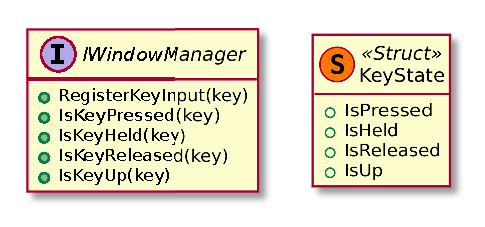
\includegraphics[width=10cm]{archivos/inputuml}
	\caption{Funciones y estructuras del sistema de input}
	\label{fig:input}
\end{figure}

\subsection{Dibujar texto}

Al igual que con el input, la necesidad de dibujar texto no se hizo aparente hasta un estado más avanzado de desarrollo del proyecto. Una vez en la tesitura en la que poder dibujar texto en pantalla era necesario, fue necesario dedicar un tiempo de análisis.\\

Inicialmente pensé en usar una librería y estuve investigando cuál podía satisfacer mejor mis objetivos. glfreetype\footnote{\url{https://github.com/benhj/glfreetype}} parecía bastante adecuada, tratándose de una librería pequeña, concisa y aparentemente sencilla de utilizar.\\

A mitad camino del proceso de integración de esta librería, no obstante, me empecé a plantear hasta qué punto tenía sentido utilizar una librería externa para el dibujado de texto en pantalla. Al fin y al cabo, uno de mis objetivos con este trabajo era que todo aquello que estuviera dibujado en pantalla hubiera sido desarrollado de forma exclusiva por mi, sin usar librerías externas. Las únicas librerías que usa este trabajo (GLFW y OpenGL) son utilizadas con el único objetivo de facilitar la implementación y no salirse del ámbito de este estudio. No obstante, este no parecía ser el caso para el dibujado de texto en pantalla.\\

No obstante, implementar un sistema de dibujado de texto parecía complejo, \emph{a priori}. Es por ello que me plantée, ¿cuál es la forma más sencilla y rápida en la que podría dibujar texto en pantalla?

Tras un tiempo de análisis, llegué a la conclusión de que implementar un sistema de dibujado de texto era una tarea sencilla y que se podía considerar dentro del ámbito de este proyecto. Por tanto, no sería necesario usar librerías externas. Este sistema de texto debería ser lo más sencillo posible, no obstante, y tendría ciertas limitaciones.\\

La mayoría de librerías de texto son capaces de leer formatos de fuente como TrueType o OpenType, además, para cada letra dibujan un \emph{quad} mediante OpenGL al que aplican una textura con transparencia representando la letra. Este proceso es más complejo de lo asumible para este proyecto, pero por suerte, no era necesario seguirlo.\\

Mi sistema estaría basado en las siguientes ideas: 
\begin{itemize}
	\item Es necesario un método para dibujar caracteres individuales
	\item Es necesario un método para dibujar cadenas de caracteres
	\item Todo lo que necesita un carácter para ser dibujado es posición, color y tamaño.
	\item La forma más sencilla de usar una fuente es crear nuestra propia fuente, que vaya embebida en el código
	\item Cualquier carácter puede ser definido dentro de una cuadrícula de 5x5 unidades como en [\ref{fontA}]
	\item No es necesario diferenciar entre mayúscula y minúscula (tener doble representación para las letras supone una pérdida de espacio y tiempo)
\end{itemize}

\begin{lstlisting}[style=C-color, caption={Método que renderiza un sólo caracter},label=fontA]
const char *Characters::A{
    "_###_"
    "#___#"
    "#####"
    "#___#"
    "#___#"
};
\end{lstlisting}

Así pues, la tareas que realmente más tiempo llevan en un sistema como el definido es crear todos los caracteres que se necesitan, que en mi caso son todas las letras del alfabeto inglés, los números y algunos caracteres especiales. Una vez hecho esto, se inserta todos estos caracteres dentro de un mapa estático cuya clave sea un caracter y el valor sea la cuadrícula 5x5 que lo representa.\\

\begin{lstlisting}[style=C-color, caption={Método que renderiza un sólo caracter},label=rendercharacter]
void ClassicDemoTemplate::RenderCharacter(char character, int x, int y, int scale, const Pixel &colour)
{
    if (character < 0 || character == ' ')
    {
        return;
    }

    const char *c = Characters::GetCharactersMap()[character];

    for (int i = x; i < x + 5 * scale; i++)
    {
        for (int j = y; j < y + 5 * scale; j++)
        {
            int offsetX = (i - x) / scale;
            int offsetY = (j - y) / scale;

            if (c[offsetY * 5 + offsetX] != ' ')
            {
                screen[j * width + i] = colour;
            }
        }
    }
}
\end{lstlisting}

Una vez tenemos el mapa de caracteres, dibujar un caracter en pantalla es de lo más sencillo [\ref{rendercharacter}]. Tras una comprobación inicial para saber si el carácter no es válido o es un espacio (que obviamente no se dibuja), lo primero que hacemos es obtener la cuadrícula 5x5 que se asocia con el caracter a dibujar.\\

Una vez hecho esto, recorremos la cuadrícula en vertical y horizontal. La cantidad de píxeles que recorremos en cada dirección es equivalente al tamaño de la cuadrícula (5) multiplicado por la escala del caracter. Así pues, un carácter con escala 1 tendrá un grosor de línea de un píxel y ocupara un espacio de 5x5 píxeles mientras que un caracter con escala 2 tendrá 2 píxeles de grosor de línea y ocupará un espacio de 10x10 píxeles.\\

Tras esto hacemos una conversión sencilla para hallar, dadas unas coordenadas cualesquiera dentro del bucle, las coordenadas de la cuadrícula que le corresponden. Una vez halladas, se comprueba la posición de la cuadrícula. Si es un espacio en blanco (en el ejemplo [\ref{fontA}] se sustituyen los espacios por barras bajas por cuestión de claridad visual) no se rellena, mientras que si esa posición de la cuadrícula no es un espacio, se pinta el píxel con el color correspondiente.\\

\begin{lstlisting}[style=C-color, caption={Método que renderiza una cadena de caracteres},label=rendertext]
void ClassicDemoTemplate::RenderText(const char *text, int posX, int posY, int scale, const Pixel &colour)
{
    std::string txt(text);
    for (auto &c : txt)
    {
        c = toupper(c);
    }

    for (auto c : txt)
    {
        RenderCharacter(c, posX, posY, scale, colour);
        posX += 6 * scale;
    }
}
\end{lstlisting}

El método para dibujar texto es también muy sencillo, como se puede ver en el ejemplo [\ref{rendertext}]. Lo primero que hacemos es poner todos los caracteres en mayúscula, pues como ya habíamos decidido antes, es más práctico tener un único conjunto de letras. A continuación, por cada caracter que forma el texto invocamos a la función de dibujado de caracter [\ref{rendercharacter}]. Por cada dibujado, aumentamos la posición horizontal, de modo que el próximo caracter se dibuje a 6 unidades de distancia del inicio del caracter anterior (es decir, se deja una unidad de 1 espacio entre uno y otro carácter, ya que un caracter ocupa 5 unidades).

\subsection{Dibujar puntos, rectángulos y líneas}

\chapter{Demos clásicas}

\section{Fuego}

\subsection{Investigación inicial}
\subsection{Planteamiento formal}
\subsection{Implementación}
\subsection{Refinamiento}
\subsection{Resultado}

\section{Geometría}

\subsection{Investigación inicial}
\subsection{Planteamiento formal}
\subsection{Implementación}
\subsection{Refinamiento}
\subsection{Resultado}

\section{Planos infinitos}

\subsection{Investigación inicial}
\subsection{Planteamiento formal}
\subsection{Implementación}
\subsection{Refinamiento}
\subsection{Resultado}

\section{Plasma}

\subsection{Investigación inicial}
\subsection{Planteamiento formal}
\subsection{Implementación}
\subsection{Refinamiento}
\subsection{Resultado}

\section{RotoZoom}

\subsection{Investigación inicial}
\subsection{Planteamiento formal}
\subsection{Implementación}
\subsection{Refinamiento}
\subsection{Resultado}

\section{Deformaciones de imagen}

\subsection{Investigación inicial}
\subsection{Planteamiento formal}
\subsection{Implementación}
\subsection{Refinamiento}
\subsection{Resultado}

\section{Túnel de puntos}

\subsection{Investigación inicial}
\subsection{Planteamiento formal}
\subsection{Implementación}
\subsection{Refinamiento}
\subsection{Resultado}

\chapter{Demo final}

\subsection{Investigación inicial}
\subsection{Planteamiento formal}
\subsection{Implementación}
\subsection{Refinamiento}
\subsection{Resultado}
		% Plantilla: Se muestran listados
%%%%%%%%%%%%%%%%%%%%%%%%%%%%%%%%%%%%%%%%%%%%%%%%%%%%%%%%%%%%%%%%%%%%%%%%
% Plantilla TFG/TFM
% Escuela Politécnica Superior de la Universidad de Alicante
% Realizado por: Jose Manuel Requena Plens
% Contacto: info@jmrplens.com / Telegram:@jmrplens
%%%%%%%%%%%%%%%%%%%%%%%%%%%%%%%%%%%%%%%%%%%%%%%%%%%%%%%%%%%%%%%%%%%%%%%%

\chapter{Conclusiones}

El bajo nivel es importante, la demoscene no debe perderse, las matemáticas son fundamentales, avanzar hacia el futuro teniendo muy presente el pasado, a veces para avanzar hay que mirar atrás, entender lo que hicieron los que iban por detrás de nosotros y saber aplicarlo	% Plantilla: Se muestran matemáticas

A test for bibliography with Xe\LaTeX.\cite{Alfonso2010a}
%%%%
% CONTENIDO. BIBLIOGRAFÍA.
%%%%
\nocite{*} %incluye TODOS los documentos de la base de datos bibliográfica sean o no citados en el texto
\bibliographystyle{unsrt}
\bibliography{bibliografia/bibliografia} % Archivo que contiene la bibliografía

%%%%
% CONTENIDO. LISTA DE ACRÓNIMOS. Comenta las líneas si no lo deseas incluir.
%%%%
% Incluye el listado de acrónimos utilizados en el trabajo. 
%\printglossary[style=modsuper,type=\acronymtype,title={Lista de Acrónimos y Abreviaturas}]
% Añade el resto de acrónimos si así se desea. Si no elimina el comando siguiente
%\glsaddallunused 

%%%%
% CONTENIDO. Anexos - Añade o elimina según tus necesidades
%%%%
%\appendix % Inicio de los apéndices
%%%%%%%%%%%%%%%%%%%%%%%%%%%%%%%%%%%%%%%%%%%%%%%%%%%%%%%%%%%%%%%%%%%%%%%%%
% Plantilla TFG/TFM
% Escuela Politécnica Superior de la Universidad de Alicante
% Realizado por: Jose Manuel Requena Plens
% Contacto: info@jmrplens.com / Telegram:@jmrplens
%%%%%%%%%%%%%%%%%%%%%%%%%%%%%%%%%%%%%%%%%%%%%%%%%%%%%%%%%%%%%%%%%%%%%%%%

\chapter{Anexo I}
Aquí vendría el anexo I 
%%%%%%%%%%%%%%%%%%%%%%%%%%%%%%%%%%%%%%%%%%%%%%%%%%%%%%%%%%%%%%%%%%%%%%%%%
% Plantilla TFG/TFM
% Escuela Politécnica Superior de la Universidad de Alicante
% Realizado por: Jose Manuel Requena Plens
% Contacto: info@jmrplens.com / Telegram:@jmrplens
%%%%%%%%%%%%%%%%%%%%%%%%%%%%%%%%%%%%%%%%%%%%%%%%%%%%%%%%%%%%%%%%%%%%%%%%


% Ejemplo de páginas en horizontal y vertical

\chapter{Páginas horizontales}
Aquí se muestra cómo incluir páginas en horizontal.

Esta página está en vertical\\
\clearpage % Nueva página

\begin{landscape} % Inicia modo horizontal
	

Esta página está en horizontal\\
\clearpage % Nueva página

Esta página también está en horizontal\\

\end{landscape} % Finaliza modo horizontal
\clearpage % Nueva página


Esta página está de nuevo en vertical\\




%%%%%%%%%%%%%%%%%%%%%%%%%%%%%%%%%%%%%%%%%%%%%%%%%%%%%%%%%%%%%%%%%%%%%%%%%
% Plantilla TFG/TFM
% Escuela Politécnica Superior de la Universidad de Alicante
% Realizado por: Jose Manuel Requena Plens
% Contacto: info@jmrplens.com / Telegram:@jmrplens
%%%%%%%%%%%%%%%%%%%%%%%%%%%%%%%%%%%%%%%%%%%%%%%%%%%%%%%%%%%%%%%%%%%%%%%%

% Ejemplo de inclusión de páginas de un PDF

\chapter{Importar PDF}

A continuación se muestra una página importada de un PDF externo. Observar los comentarios en el código de este anexo para más información. También puedes leer el manual con todas las opciones en \url{http://osl.ugr.es/CTAN/macros/latex/contrib/pdfpages/pdfpages.pdf}.

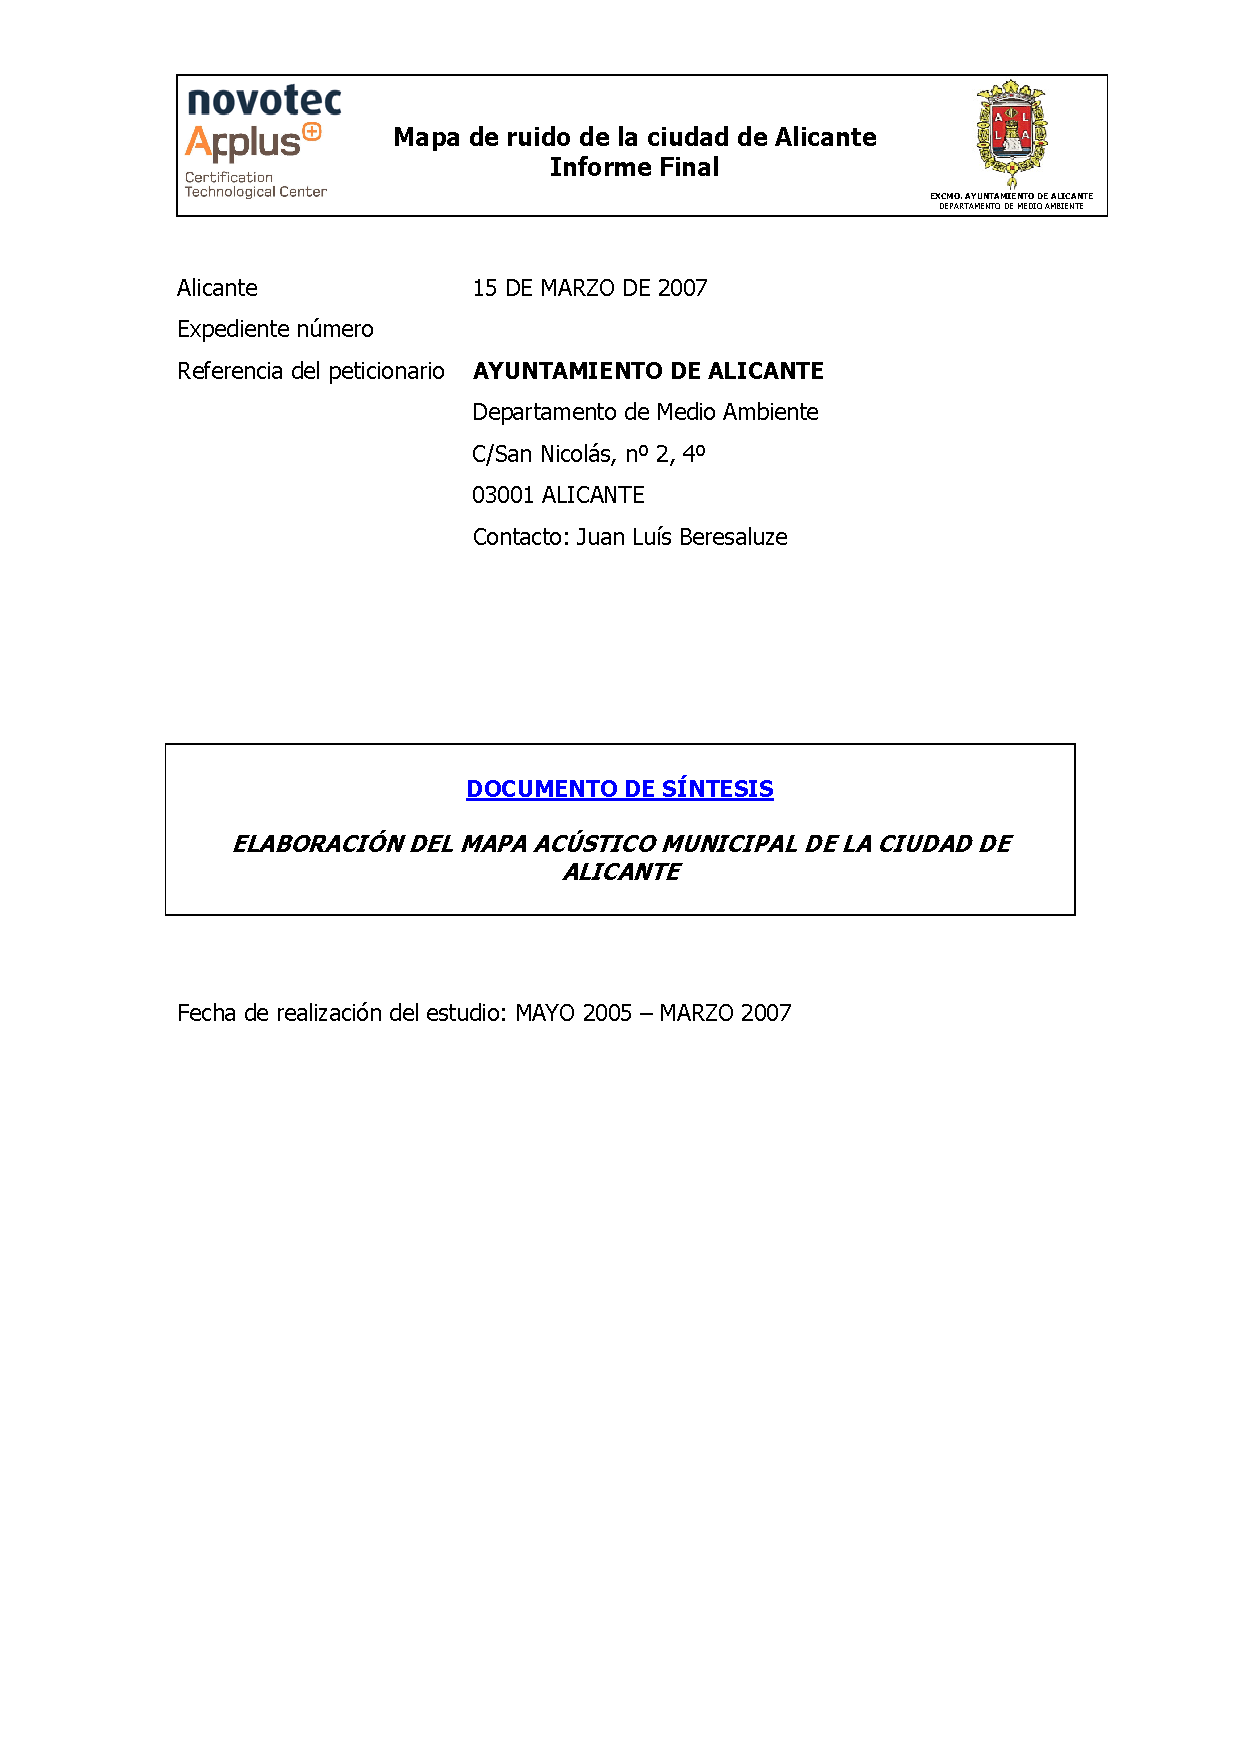
\includepdf[pages={1}]{archivos/ES_a_DF7_Agg_Alicante.pdf}

% Para incluir una página:
% [pages={0}] % Donde '0' es el número de la pagina del PDF que se quiere incluir

% Para incluir varias páginas consecutivas
% [pages={1-4}] % Con estos valores importa de la página 1 a la 4.

% Para incluir varias páginas salteadas
% [pages={1,4,7,10}] % Incluye las páginas 1,4,7 y 10

% Para incluir todo el documento PDF
% [pages=-]

% Si ademas de pages=... se incluye landscape, se importa en horizontal
% [pages{1},landscape]

\end{document}
